% +--------------------------------------------------------------------+
% | LaTeX Template for K-State Electronic Theses, Dissertations,
% | and Reports
% |
% | Some guidelines for using the template are shown in comments.  Read
% | these comments carefully, as they describe changes you will need to
% | make to the template in order to meet Graduate School requirements.            |
% |
% | Additional information on using the template are contained in these
% | files, which are included when you download the template:
% |
% | ReadMe.pdf - A general overview of using the template
% |
% | BibTeX Guide.pdf - Detailed guidelines on using BibTeX to create
% | your bibliography and manage your citations.
% |
% | natbib.pdf - Gives detailed information on using the natbib package
% | and formatting citations
% +--------------------------------------------------------------------+

% +--------------------------------------------------------------------+
% | The template is designed to be used with PDFLaTeX. Process this
% | file (etdrtemplate.tex) with PDFLaTeX in order to produce a PDF
% | version of your ETDR.  If you are using BibTex to manage your
% | refrences, you will need to process your file four times:
% | 1. Run PDFLaTeX
% | 2. Run BibTex
% | 3. Run PDFLaTeX
% | 4. Run PDFLaTeX
% |
% | Some LaTeX editors do not explicitly list PDFLaTeX as an option, but
% | do use PDFLaTeX to produce a PDF file directly from your .tex files.
% | See the ReadMe file for details.
% +--------------------------------------------------------------------+
% |
% +--------------------------------------------------------------------+
% |
% | As required by the Graduate School, The template is configured to
% | contain the following sections in the order shown.

% | Abstract title page (doctoral dissertations only)
% | Abstract (doctoral dissertations only)
% | Title page
% | Copyright page
% | Abstract
% | Table of contents
% | List of figures
% | List of tables
% | Acknowledgements (Optional)
% | Dedication (Optional)
% | Preface (Optional)
% | Individual Chapters
% | References or Bibliography
% | Appendices (as needed)
% |
% | Details on removing optional sections are given in the comments below.
% |
% +--------------------------------------------------------------------+

% +--------------------------------------------------------------------+
% | The LaTex command \documentclass selects a particular class to
% | associate with the document.  Within this command, 12pt is
% | specified for the font size.  You can change this to 11 pt, if
% | desired.
% +--------------------------------------------------------------------+

\documentclass[final,letterpaper,12pt,oneside]{class_diss}

% +--------------------------------------------------------------------+
% | Here are added external packages that will be used throughout
% | the document.  You can add other packages as needed.
% +--------------------------------------------------------------------+

\usepackage{graphicx} % Extended graphics package.
\usepackage{amsmath} % American Mathematics Society standards
\usepackage{amsxtra} % Additional math symbols
\usepackage{amssymb} % Additional math symbols
\usepackage{amsthm} % Additional math symbols
\usepackage{latexsym} % Additional math symbols
\usepackage{setspace} % Controls line spacing
\usepackage[margin=1in]{geometry} % Sets page margins to 1 inch on all sides
\usepackage[titles]{tocloft} % Adds leader dots to all entries in the table of contents
%\usepackage{parskip} 

% Already included below
%\usepackage{hyperref} % to include hyperlinks in appendix

% For matlab code
\usepackage{listings}
\usepackage{color} %red, green, blue, yellow, cyan, magenta, black, white
\definecolor{mygreen}{RGB}{53,95,58} % color values Red, Green, Blue
\definecolor{mylilas}{RGB}{170,55,241}

% To manage acronyms
\usepackage{acronym}

% Blank line between paragraphs while keeping indents
%\edef\restoreparindent{\parindent=\the\parindent\relax}
%\usepackage{parskip}
%\restoreparindent

% To have table and figures on same row
\usepackage{floatrow}
% Table float box with bottom caption, box width adjusted to content
\newfloatcommand{capbtabbox}{table}[][\FBwidth]

\usepackage[font=small,labelfont=bf,tableposition=top]{caption}
\DeclareCaptionLabelFormat{andtable}{#1~#2  \&  \tablename~\thetable}

% +--------------------------------------------------------------------+
% |
% | Citation and Bibliography Style
% |
% | The following commands determine the citation and bibliography style.  The
% | template uses BibTeX for formatting the bibliography.  See "BibTeX Guide.pdf"
% | for details on formatting citations and references.  The template is set
% | to use a generic, superscript style, but it can be easily modified
% | to use author-year styles.

\bibliographystyle{unsrtnat}
% | If you want to use an author-year citation style, change "unsrtnat" to
% | "plainnat" in the line above.  You can also use other styles supported
% | by LaTeX, e.g., acm, ieeetr, siam, etc.  Additional styles
% | are in the \styles folder and can be invoked like this:
% | \bibliographystyle{styles/apsrev}.  If the style you use is based
% | on an author-year citation style, you will need to make changes
% | in the usepackage and \setcitestyle statements below

\usepackage[super,sort&compress]{natbib}
% | If you want to use an author-year citation style, change "super" to
% | "authoryear" in the line above.

\setcitestyle{super}
% | if you want to use an author-year citation style, change "super" to
% | "authoryear" in the line above.

% +---------------------------------------------------------------------+
% | The hyperref package enables cross-references.
% +---------------------------------------------------------------------+

\usepackage[pdftex, plainpages=false, pdfpagelabels]{hyperref}

\hypersetup{
    linktocpage=true,
    colorlinks=true,
    bookmarks=true,
    citecolor=blue,
    urlcolor=blue,
    linkcolor=blue,
    citebordercolor={1 0 0},
    urlbordercolor={1 0 0},
    linkbordercolor={.7 .8 .8},
    breaklinks=true,
    pdfpagelabels=true,
    }

% +--------------------------------------------------------------------+
% | The document begins here.
% +--------------------------------------------------------------------+

\doublespacing
\begin{document}

% +--------------------------------------------------------------------+
% | ******Masters Students -- You Need to Make Some Changes Here******
% |
% | The Abstract Title page and Abstract page following the Abstract
% | Title page are required only for doctoral dissertations.  For
% | masters theses or reports, comment out or delete the lines:
% |
% | % +--------------------------------------------------------------------+
% | Abstract Title Page
% |
% |This page is required only for doctoral dissertations.
% +--------------------------------------------------------------------+

% +--------------------------------------------------------------------+
% | This page should not contain a page number.  We use the
% | \thispagestyle[empty] command below to suppress page numbers
% | and other style elements.
% +--------------------------------------------------------------------+

\thispagestyle{empty}

% +--------------------------------------------------------------------+
% | The Abstract Title page begins here
% +--------------------------------------------------------------------+

\pdfbookmark[0]{Title Page}{PDFTitlePage}
%\setcounter{page}{1}

\begin{center}

   \vspace{1cm}

% +--------------------------------------------------------------------+
% | Enter the title of your ETDR below.  Use ALL CAPITAL LETTERS.
% +--------------------------------------------------------------------+

   \large ENTER YOUR TITLE\\

   \vspace{0.5cm}

   by\\

   \vspace{0.5cm}

% +--------------------------------------------------------------------+
% | Enter your name below in ALL CAPITAL LETTERS.
% +--------------------------------------------------------------------+

   \large ENTER YOUR NAME\\

   \vspace{0.5cm}

% +--------------------------------------------------------------------+
% | On the line below, replace "Enter Your Previous Degrees"
% | with your previous degrees in mixed case. Include the abbreviation
% | for the degree, the name of the university, and the year separated
% | by commas. For example:
% |
% |    B.A., University of Illinois, 2000
% |
% | If desired, it is acceptable to include a city or country with
% | the university name. For example:
% |
% |    B.S., Jillian University, China, 2002
% |
% | Each degree should appear on a separate line.  Use the \\
% | command to create a line break.
% +--------------------------------------------------------------------+

   Enter Your Previous Degrees\\

   \vspace{0.55cm}
   \rule{2in}{0.5pt}\\
   \vspace{0.75cm}

   {\large AN ABSTRACT OF A DISSERTATION}\\

   \vspace{0.5cm}
   \begin{singlespace}
   submitted in partial fulfillment of the\\
   requirements for the degree\\
   \end{singlespace}

   \vspace{0.5cm}

% +--------------------------------------------------------------------+
% | On the line below, enter the name of your earned degree in ALL
% | CAPITAL LETTERS.  For example: DOCTOR OF PHILOSOPHY
% +--------------------------------------------------------------------+


   {\large ENTER YOUR DEGREE NAME}\\
   \vspace{0.5cm}

% +--------------------------------------------------------------------+
% | On the two lines below, enter the name of your department and the
% | name of the college in mixed case.  For example:
% |
% |     Biochemistry Department
% |     College of Arts and Sciences
% +--------------------------------------------------------------------+

   \begin{singlespace}
   Enter Your Department Name\\
   Enter Your College Name\\
   \end{singlespace}

   \vspace{0.5cm}

   \begin{singlespace}
   {\Large KANSAS STATE UNIVERSITY}\\
   Manhattan, Kansas\\
   \end{singlespace}

% +--------------------------------------------------------------------+
% | On the line below, replace "Graduation Year" with the four-digit year
% | of your graduation. For example:
% |
% |     2016
% +--------------------------------------------------------------------+

   Graduation Year\\
   \vspace{1cm}

\end{center}
 through \end{abstract}.
% |
% | You will also need to uncomment the two lines following the
% | \begin{abstract} command:
% |    %\setcounter{page}{-1}
% |    %\pdfbookmark[0]{Abstract}{PDFAbstractPage}
% |
% | Don't uncomment the lines above.  Scroll down several lines until
% | you see the section "For masters theses or reports, uncomment
% | the commands..." and uncomment the lines in that section.
% +--------------------- ----------------------------------------------+

%% +--------------------------------------------------------------------+
% | Abstract Title Page
% |
% |This page is required only for doctoral dissertations.
% +--------------------------------------------------------------------+

% +--------------------------------------------------------------------+
% | This page should not contain a page number.  We use the
% | \thispagestyle[empty] command below to suppress page numbers
% | and other style elements.
% +--------------------------------------------------------------------+

\thispagestyle{empty}

% +--------------------------------------------------------------------+
% | The Abstract Title page begins here
% +--------------------------------------------------------------------+

\pdfbookmark[0]{Title Page}{PDFTitlePage}
%\setcounter{page}{1}

\begin{center}

   \vspace{1cm}

% +--------------------------------------------------------------------+
% | Enter the title of your ETDR below.  Use ALL CAPITAL LETTERS.
% +--------------------------------------------------------------------+

   \large ENTER YOUR TITLE\\

   \vspace{0.5cm}

   by\\

   \vspace{0.5cm}

% +--------------------------------------------------------------------+
% | Enter your name below in ALL CAPITAL LETTERS.
% +--------------------------------------------------------------------+

   \large ENTER YOUR NAME\\

   \vspace{0.5cm}

% +--------------------------------------------------------------------+
% | On the line below, replace "Enter Your Previous Degrees"
% | with your previous degrees in mixed case. Include the abbreviation
% | for the degree, the name of the university, and the year separated
% | by commas. For example:
% |
% |    B.A., University of Illinois, 2000
% |
% | If desired, it is acceptable to include a city or country with
% | the university name. For example:
% |
% |    B.S., Jillian University, China, 2002
% |
% | Each degree should appear on a separate line.  Use the \\
% | command to create a line break.
% +--------------------------------------------------------------------+

   Enter Your Previous Degrees\\

   \vspace{0.55cm}
   \rule{2in}{0.5pt}\\
   \vspace{0.75cm}

   {\large AN ABSTRACT OF A DISSERTATION}\\

   \vspace{0.5cm}
   \begin{singlespace}
   submitted in partial fulfillment of the\\
   requirements for the degree\\
   \end{singlespace}

   \vspace{0.5cm}

% +--------------------------------------------------------------------+
% | On the line below, enter the name of your earned degree in ALL
% | CAPITAL LETTERS.  For example: DOCTOR OF PHILOSOPHY
% +--------------------------------------------------------------------+


   {\large ENTER YOUR DEGREE NAME}\\
   \vspace{0.5cm}

% +--------------------------------------------------------------------+
% | On the two lines below, enter the name of your department and the
% | name of the college in mixed case.  For example:
% |
% |     Biochemistry Department
% |     College of Arts and Sciences
% +--------------------------------------------------------------------+

   \begin{singlespace}
   Enter Your Department Name\\
   Enter Your College Name\\
   \end{singlespace}

   \vspace{0.5cm}

   \begin{singlespace}
   {\Large KANSAS STATE UNIVERSITY}\\
   Manhattan, Kansas\\
   \end{singlespace}

% +--------------------------------------------------------------------+
% | On the line below, replace "Graduation Year" with the four-digit year
% | of your graduation. For example:
% |
% |     2016
% +--------------------------------------------------------------------+

   Graduation Year\\
   \vspace{1cm}

\end{center}
  % Masters students - comment or delete this line

%\begin{abstract} % Masters students - comment or delete this line
%   \setcounter{page}{-1} % Masters students - comment or delete this line
%   \pdfbookmark[0]{Abstract}{PDFAbstractPage} % Masters students - comment or delete this line
%   % +--------------------------------------------------------------------+
% | Abstract Page
% +--------------------------------------------------------------------+

\pagestyle{empty}
%\vspace{1cm}
\setlength{\baselineskip}{0.8cm}

%\indent

% +--------------------------------------------------------------------+
% | Enter the text of your abstract below, maximum of 500 words.
% +--------------------------------------------------------------------+


Developments in farm related technology have increased the importance of mapping individual plants in the field.  An automated mapping process allows the size of these fields to scale up without being hindered by time-intensive, manual surveying.  This research focuses on the development of a mapping process, which uses geo-located images of the field to automatically locate plants and determine their coordinates.  Additionally, this mapping process is capable of differentiating between groupings of plants by using Quick Response (QR) codes.  This research applies to plants that have been grown into seedlings before being planted, known as transplants, in a standard row configuration. 

The development of this mapping process is presented in two stages.  First is the design of a platform capable of traversing the field and capturing images, and second is the post-processing steps which convert the images into a field map.  This mapping system was applied to a field at the Land Institute containing roughly 25,000 plants. The results show the mapped plant locations are accurate to within a few inches, and the use of QR codes is effective for identifying plant groups.  These results demonstrate this method is successful in mapping large fields.  However, the high overall complexity makes the system restrictive for smaller fields, where a simpler, semi-automated solution is preferable. An example of such a system is presented at the conclusion of the thesis.
 % Masters students - comment or delete this line
%   \vfill % Masters students - comment or delete this line
%\end{abstract} % Masters students - comment or delete this line

% +--------------------------------------------------------------------+
% | Title Page -- Required for both Doctoral and Masters Students
% +--------------------------------------------------------------------+

% +--------------------------------------------------------------------+
% | Title Page
% +--------------------------------------------------------------------+

\newpage

% +--------------------------------------------------------------------+
% | This page should not contain a page number.  We use the
% | \thispagestyle[empty] command below to suppress page numbers
% | and other style elements.
% +--------------------------------------------------------------------+

\thispagestyle{empty}

% +--------------------------------------------------------------------+
% | The Title page begins here.
% +--------------------------------------------------------------------+

\begin{center}

   \vspace{1cm}

% +--------------------------------------------------------------------+
% | On the line below, replace "ENTER YOUR TITLE" with the title of
% | your ETDR.  Use all CAPITAL LETTERS.
% +--------------------------------------------------------------------+

   \large IMAGE-BASED MAPPING PROCESS FOR \\
   TRANSPLANTED SEEDLINGS\\

   \vspace{0.3cm}

   by\\

   \vspace{0.3cm}

% +--------------------------------------------------------------------+
% | On the line below, replace "ENTER YOUR NAME" with your name.  Use
% | mixed case, for example, Laura Bush.
% +--------------------------------------------------------------------+

   \large Kyle McGahee\\

   \vspace{0.3cm}

% +--------------------------------------------------------------------+
% | On the line below, replace "Enter Your Previous Degrees"
% | with your previous degrees in mixed case. Include the abbreviation
% | for the degree, the name of the university, and the year separated
% | by commas. For example:
% |
% |    B.A., University of Illinois, 2000
% |
% | If desired, it is acceptable to include a city or country with
% | the university name. For example:
% |
% |    B.S., Jillian University, China, 2002
% |
% | Each degree should appear on a separate line.  Use the \\
% | command to create a line break.
% +--------------------------------------------------------------------+

   B.S., Kansas State University, 2014\\

   \vspace{0.35cm}
   \rule{2in}{0.5pt}\\
   \vspace{0.65cm}

   {\large A THESIS}\\

   \vspace{0.3cm}
   \begin{singlespace}
   submitted in partial fulfillment of the\\
   requirements for the degree\\
   \end{singlespace}

   \vspace{0.3cm}

% +--------------------------------------------------------------------+
% | On the line below, replace "ENTER YOUR DEGREE NAME" with the name
% | of your earned degree in ALL CAPITAL LETTERS.
% +--------------------------------------------------------------------+

   {\large MASTER OF SCIENCE}\\
   \vspace{0.3cm}

% +--------------------------------------------------------------------+
% | On the two lines below, replace "Enter Your Department Name" and
% | "Enter Your College Name" with the name of your department and the
% | name of the college in mixed case.  For example:
% |
% |     Biochemistry Department
% |     College of Arts and Sciences
% +--------------------------------------------------------------------+

   \begin{singlespace}
   Department of Mechanical and Nuclear Engineering\\
   College of Engineering\\
   \end{singlespace}

   \vspace{0.3cm}

   \begin{singlespace}
   {\large KANSAS STATE UNIVERSITY}\\
   Manhattan, Kansas\\
   \end{singlespace}

% +--------------------------------------------------------------------+
% | On the line below, replace "Graduation Year" with the four-digit
% | year of your graduation.  For example:
% |
% |     2016
% +--------------------------------------------------------------------+

   2016\\
   \vspace{0.3cm}

    \end{center}

    \begin{flushright}
    Approved by:\\
    \vspace{0.3cm}
    \begin{singlespace}
    Major Professor


% +--------------------------------------------------------------------+
% | On the line below, replace "Enter Your Major Professor's Name"
% | with  the name of your major professor in mixed case.  Use the
% | format Firstname Lastname.  For example:
% |
% |     Lori Goetsch
% |
% +--------------------------------------------------------------------+

    Dr. Dale Schinstock\\
    \end{singlespace}
    \end{flushright}

% +--------------------------------------------------------------------+
% | If you have co-major professors, comment out the lines above from
% | \begin{flushright} through \end{flushright} and uncomment the
% | lines below.  Enter your co-major professors' names where indicated.
% +--------------------------------------------------------------------+

%\begin{flushright}
%   Approved by:\\
%  \vspace{ 0.3cm}
%   \begin{singlespace}
%   Co-Major Professor\\
%   Enter Your Co-Major Professor's Name\\
%   \vspace{.25cm}
%   Co-Major Professor\\
%   Enter Your Co-Major Professor's Name\\
%   \end{singlespace}
%\end{flushright}


% +--------------------------------------------------------------------+
% | Copyright Page -- Required for both Doctoral and Masters Students
% +--------------------------------------------------------------------+

% +--------------------------------------------------------------------+
% | Copyright Page
% +--------------------------------------------------------------------+

\newpage

\thispagestyle{empty}

\vspace*{0.9cm}

\begin{center}

{\bf \Huge Copyright}

\vspace{1cm}

% +--------------------------------------------------------------------+
% | On the line below, replace "Enter Your Name" with your name
% | Use the same form of your name as it appears on your title page.
% | Use mixed case, for example, Barack Obama.
% +--------------------------------------------------------------------+

   \Large Kyle McGahee\\

   \vspace{0.5cm}

% +--------------------------------------------------------------------+
% | On the line below, replace "Graduation Year" with the four-digit year
% | of your graduation. For example:
% |
% |     2016
% |
% +--------------------------------------------------------------------+

   2016\\

   \vspace{0.5cm}

\end{center}


% +--------------------------------------------------------------------+
% |  Abstract -- Required for both Doctoral and Masters Students
% +--------------------------------------------------------------------+

\begin{abstract}

% +--------------------------------------------------------------------+
% | For masters theses or reports, uncomment the commands on the next
% | two lines (\setcounter and \pdfbookmark)
% +--------------------------------------------------------------------+

   \setcounter{page}{-1}
   \pdfbookmark[0]{Abstract}{PDFAbstractPage}

% +--------------------------------------------------------------------+
% | Abstract Page
% +--------------------------------------------------------------------+

\pagestyle{empty}
%\vspace{1cm}
\setlength{\baselineskip}{0.8cm}

%\indent

% +--------------------------------------------------------------------+
% | Enter the text of your abstract below, maximum of 500 words.
% +--------------------------------------------------------------------+


Developments in farm related technology have increased the importance of mapping individual plants in the field.  An automated mapping process allows the size of these fields to scale up without being hindered by time-intensive, manual surveying.  This research focuses on the development of a mapping process, which uses geo-located images of the field to automatically locate plants and determine their coordinates.  Additionally, this mapping process is capable of differentiating between groupings of plants by using Quick Response (QR) codes.  This research applies to plants that have been grown into seedlings before being planted, known as transplants, in a standard row configuration. 

The development of this mapping process is presented in two stages.  First is the design of a platform capable of traversing the field and capturing images, and second is the post-processing steps which convert the images into a field map.  This mapping system was applied to a field at the Land Institute containing roughly 25,000 plants. The results show the mapped plant locations are accurate to within a few inches, and the use of QR codes is effective for identifying plant groups.  These results demonstrate this method is successful in mapping large fields.  However, the high overall complexity makes the system restrictive for smaller fields, where a simpler, semi-automated solution is preferable. An example of such a system is presented at the conclusion of the thesis.

\vfill
\end{abstract}

% +--------------------------------------------------------------------+
% | The following commands start a new page and set the page numbering
% | to lowercase roman numerals.
% +--------------------------------------------------------------------+

\newpage
\pagenumbering{roman}

% +--------------------------------------------------------------------+
% |
% | *********************** IMPORTANT ******************************
% |
% | In the \setcounter command below, set the number to represent the
% | page number of the table of contents page.  For example, if the
% | table of contents page is the 6th page of your document, enter 6
% | in the brackets.  This number may vary, depending on the length of
% | your abstract.
% |
% | Numbers do not appear on the title and abstract pages, but they
% | are included in the page count.  The table of contents page is the
% | first page on which page numbers are displayed.
% +--------------------------------------------------------------------+

\setcounter{page}{4}

% +--------------------------------------------------------------------+
% | The following command creates a bookmark for the table of contents
% | in the final PDF document.
% +--------------------------------------------------------------------+

\pdfbookmark[0]{\contentsname}{contents}

% +--------------------------------------------------------=-----------+
% | The following command adds dot leaders for all entries in the
% | table of contents.
% +--------------------------------------------------------------------+

\renewcommand{\cftchapleader}{\cftdotfill{\cftdotsep}}

% +--------------------------------------------------------------------+
% | The following commands makes all entries and page numbers in the
% | table of contents appear in normal weight font (not bold).
% +--------------------------------------------------------------------+

\renewcommand{\cftchapfont}{\mdseries}
\renewcommand{\cftchappagefont}{\mdseries}

% +--------------------------------------------------------------------+
% | These commands add the table of contents, list of figures, and
% | list of tables.
% +--------------------------------------------------------------------+

\tableofcontents
\listoffigures
\listoftables

% +--------------------------------------------------------------------+
% | Acronyms Page
% +--------------------------------------------------------------------+

\newpage
\phantomsection
\addcontentsline{toc}{chapter}{Acronyms}
% +--------------------------------------------------------------------+
% | Acronyms Page 
% +--------------------------------------------------------------------+

%\newpage
\vspace*{0.2cm}
\begin{center}
{\bf \Huge Acronyms}
\end{center}

\begin{acronym}[EDSDK12] % longest acro

% Single space
\setlength{\parskip}{0ex}
\setlength{\itemsep}{0ex}

\acro{apsc}[APSC]{Advanced Photo System Type-C}
\acro{bgr}[BGR]{Blue Green Red}
\acro{csv}[CSV]{Comma Separated Value}
\acro{dslr}[DSLR]{Digital Single-Lens Reflex}
\acro{edsdk}[EDSDK]{EOS Digital Software Development Kit}
\acro{fpga}[FPGA]{Field Programmable Gate Array}
\acro{gnss}[GNSS]{Global Navigation Satellite System}
\acro{gps}[GPS]{Global Positioning System}
\acro{hsv}[HSV]{Hue Saturation Value}
\acro{imu}[IMU]{Inertial Measurement Unit}
\acro{iso}[ISO]{International Standards Organization}
\acro{jpg}[JPEG]{Joint Photographic Experts Group}
\acro{led}[LED]{Light Emitting Diode}
\acro{lidar}[LiDAR]{Light Detection and Ranging}
\acro{qr}[QR]{Quick Response}
\acro{ros}[ROS]{Robot Operating System}
\acro{rtk}[RTK]{Real Time Kinematic}
\acro{sse}[SSE]{Sum of Squared Errors}
\acro{ssh}[SSH]{Secure Shell}
\acro{url}[URL]{Uniform Resource Locator}
\acro{usb}[USB]{Universal Serial Bus}
\acro{utm}[UTM]{Universal Transverse Mercator}
\acro{utc}[UTC]{Coordinated Universal Time}
\acro{wgs}[WGS-84]{World Geodetic System}

\end{acronym}

%\begin{acronym}[CSSK] % longest acro

%\acro{css2}[CSS]{Customer Support Service}
%\acro{css1}[CSSK]{Customer Support Service Kyle}

%\end{acronym}

%Examples:
%\newline ac   \ac{css2}
%\newline ac   \ac{css2} 
%\newline acf  \acf{css2} 
%\newline acs  \acs{css2} 
%\newline acl  \acl{css2} 
%\newline acp \acp{css2}

% +--------------------------------------------------------------------+
% | Acknowledgements Page
% |
% | If you choose not to have an Acknowledgements page, comment out
% | or delete the following 3 lines.
% +--------------------------------------------------------------------+

\newpage
\phantomsection
\addcontentsline{toc}{chapter}{Acknowledgements}
% +--------------------------------------------------------------------+
% | Acknowledgements Page (Optional)
% +--------------------------------------------------------------------+

%\newpage
\vspace*{0.9cm}
\begin{center}
{\bf \Huge Acknowledgments}
\end{center}

\setlength{\baselineskip}{0.8cm}

%\pdfbookmark[0]{Acknowledgements}{PDF_Acknowledgements}

% +--------------------------------------------------------------------+
% | Enter text for your acknowledgements in the space below this box.
% |                                                                    
% +--------------------------------------------------------------------+

I would like to thank Dr. Jesse Poland and the National Science Foundation for the opportunity to complete this research.  Dr. Dale Schinstock for being a great mentor and always keeping me pointed in the right direction on my studies.  Ethan Wells for helping in the development of the data collection program.  Dr. Kevin Wang for his work on the first version of the camera triggering interface.  Josh Sharon for welding the top frame attached to the robot, and Byron Evers for helping me transport the robot to Salina.   Most importantly I'd like to thank my loving parents and sisters, because without them I wouldn't be anywhere close to where I am today.


% +--------------------------------------------------------------------+
% | Dedication Page
% |
% | If you choose not to have a Dedication page, comment out
% | or delete the following 3 lines.
% +--------------------------------------------------------------------+

%\newpage
%\phantomsection
%\addcontentsline{toc}{chapter}{Dedication}
%% +--------------------------------------------------------------------+
% | Dedication Page (Optional)
% +--------------------------------------------------------------------+

%\newpage
\vspace*{0.9cm}
\begin{center}
{\bf \Huge Dedication}
\end{center}

\setlength{\baselineskip}{0.8cm}

%\pdfbookmark[0]{Dedication}{PDF_Dedication}

% +--------------------------------------------------------------------+
% | Enter the text for your dedication in the space below this box.    
% +--------------------------------------------------------------------+

Enter the text for your Dedication page in the dedication.tex file.
The Dedication page is optional.  If you wish to remove it, see the
comments in the etdrtemplate.tex file.


% +--------------------------------------------------------------------+
% | Preface Page
% |
% | If you choose not to have a Dedication page, comment out
% | or delete the following 3 lines.
% +--------------------------------------------------------------------+

%\phantomsection
%\addcontentsline{toc}{chapter}{Preface}
%% +--------------------------------------------------------------------+
% | Preface (Optional)
% +--------------------------------------------------------------------+

\newpage
\vspace*{0.9cm}
\begin{center}
{\bf \Huge Preface}
\end{center}

\setlength{\baselineskip}{0.8cm}

%\pdfbookmark[0]{Preface}{PDF_Preface}

% +--------------------------------------------------------------------+
% | Enter text of your Preface in the space below this box.            
% +--------------------------------------------------------------------+

Enter the text for your Preface page in the preface.tex file. The
Preface page is optional.  If you wish to remove it, see the
comments in the etdrtemplate.tex file.



% +--------------------------------------------------------------------+
% | This is where the chapter content of your ETDR begins.
% +--------------------------------------------------------------------+

%\phantomsection
\newpage
\pagenumbering{arabic}
\setcounter{page}{1}

% +--------------------------------------------------------------------+
% | Individual chapters of your ETDR are added using the \input
% | command.
% +--------------------------------------------------------------------+

%% +--------------------------------------------------------------------+
% | Sample Chapter 1
% |
% | This file provides examples of how to
% | - insert a figure with a caption
% | - construct a table with a caption
% | - create subsections within the chapter
% | - insert a reference to a Figure or Table
% | - make a citation
% +--------------------------------------------------------------------+

\cleardoublepage

% +--------------------------------------------------------------------+
% | Replace "Chapter Title" below with the title of your chapter.
% | LaTeX will automatically number the chapters.
% +--------------------------------------------------------------------+

\chapter{Chapter Title}
\label{makereference1}

In this chapter there examples of various features you may want to
incorporate into your document. Here's an example of a figure
inserted into the text:

\begin{figure}[htb]%t=top, b=bottom, h=here

    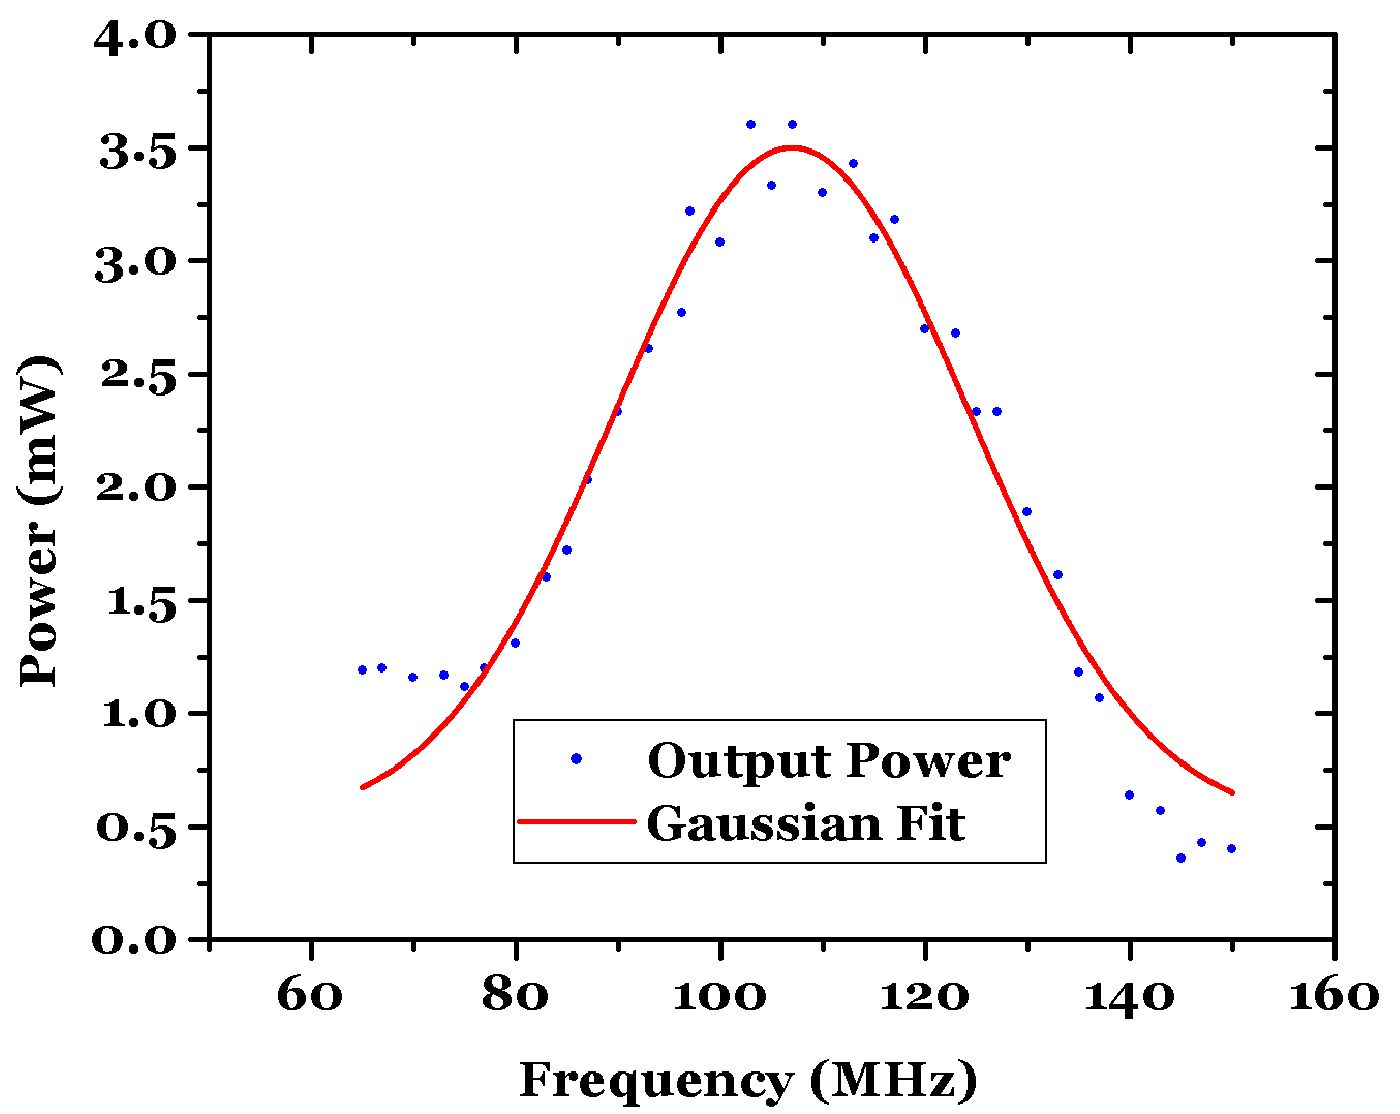
\includegraphics[height=2.5in]{figures/graph.jpg}

    \caption[Optional: Short caption to appear in List of
    Figures]{Full caption to appear below the Figure}

    \label{figure1}
\end{figure}

% +--------------------------------------------------------------------+
% |To create cross-references to figures, tables and segments
% |of text, LaTeX provides the following commands:
% |   \label{marker}
% |   \ref{marker}
% |   \pageref{marker}
% | where {marker} is a unique identifier.
% |
% | In the line above, we use \label{figure1} to mark a location
% | we wish to refer to later.  LATEX replaces \ref by the number of
% | the chapter, section, subsection, figure, or table after which the
% | corresponding \label command was issued. \pageref prints the page
% | number of the page where the \label command occurred.
% |
% +--------------------------------------------------------------------+

See the file chapter1.tex for examples of the commands used to
insert a figure or table, add a caption, etc.  Here is an example of
a table:

\begin{table}[ht]

% +--------------------------------------------------------------------+
% | We include the command \begin{center} to center the table
% | horizontally on the page.  Note use of the command \end{center}
% | to turn off centering after the table is defined.
% +--------------------------------------------------------------------+
    \begin{center}

% +--------------------------------------------------------------------+
% | The table is created with this command
% |
% | \begin{tabular}[pos]{table spec}
% |
% | The "pos" argument specifies the vertical position of the table
% | relative to the baseline of the surrounding text.  Use t, b, or c
% | to specify alignment at the top, bottom, or center.
% |
% | The "table spec" command defines the format of the table
% |   l for a column of left-aligned text
% |   r for a column of right-aligned text
% |   c for centered text
% |   p{width} for a column containing justified text with line breaks
% |   | for a vertical line
% |
% |  In this example, the caption is made to appear above the table
% |  by positioning the \caption command before the \begin{tabular
% |  command. To position the caption below the table, insert the
% |  \caption command after the \end{tabular} command.
% +--------------------------------------------------------------------+
    \caption{Caption to appear above the table}
    \begin{tabular}[c]{|c|c|c|}
        \hline
        Column 1 Heading & Column 2 Heading & Column 3 Heading \\
        \hline
        Col 1 Row 1 & Col 2 Row 1 & Col 3 Row 1\\
        Col 1 Row 2 & Col 2 Row 2 & Col 3 Row 2\\
        Col 1 Row 3 & Col 2 Row 3 & Col 3 Row 3\\
        \hline
    \end{tabular}

    \label{table1}
   \end{center}
\end{table}



% +--------------------------------------------------------------------+
% | Replace \section headings below with the title of your
% | subsections.  LaTeX will automatically number the subsections 1.1,
% | 1.2, 1.3, etc.
% +--------------------------------------------------------------------+

\section{Making References to Figures or Tables}
\label{makereference1.1}

It is possible to create cross-references and hyperlinks to items or
sections within your paper.  For example, here is a reference to
Fig.~\ref{figure1} mentioned at the beginning of this chapter and a
reference to the Table~\ref{table1}.

\section{Making a Reference to a Chapter Subsection}
\label{makereference1.2}

In this section, we refer back to text mentioned in
Section~\ref{makereference1.1} on page~\pageref{makereference1.1}.

\section{Making a Citation}
\label{makereference1.3}

Here's an example of a citation to a single
work.~\citep{CT:Weiner:1999} It's also possible to make multiple
citations.~\citep{CT:Phillips:1985, ARP:Loy:1974}

This template uses BibTeX to manage and format citations.  BibTeX is
not the only way to create a bibliography within LaTeX, but it's
generally considered to be the best option for long documents like a
thesis or dissertation.~\citep{CT:Gould:1988}  There are a few more
sample citations in this paragraph so you can see examples of how
in-text references are made and how the bibliography is
formatted.~\citep{ARP:Melinger:1991} See the file "BibTeX Guide.pdf"
for information on how to use BibTeX.

%% +--------------------------------------------------------------------+
% | Sample Chapter 2
% +--------------------------------------------------------------------+

\cleardoublepage

% +--------------------------------------------------------------------+
% | Replace "This is Chapter 2" below with the title of your chapter.
% | LaTeX will automatically number the chapters.                      
% +--------------------------------------------------------------------+

\chapter{This is Chapter 2}
\label{makereference2}

To refer to Chapter~\ref{makereference1}, use the slash ref command
along with the "makereference" label which was assigned back at the
beginning of Chapter 1.

\section{Page Number References}
\label{makereference2.1} It is possible to refer to a specific page
number, such as page~\pageref{makereference1}.  Add a slash label
command and a unique name for each page to be referenced later in
the text.

\section{Referring to Sections Within Chapter 1}
\label{makereference2.2} It is possible to refer to sections within
a chapter.  Add a slash label command and a unique name with the
section number for each section to be referenced later in the text.
Her is an example of a figure in section~\ref{makereference1.1} and
an example of a table in section~\ref{makereference1.2}.  In
section~\ref{makereference1.3}, we looked at examples of
bibliographic citations.

%% +--------------------------------------------------------------------+
% | Sample Chapter 3
% +--------------------------------------------------------------------+

\cleardoublepage

% +--------------------------------------------------------------------+
% | Replace "This is Chapter 3" below with the title of your chapter.
% | LaTeX will automatically number the chapters.                      
% +--------------------------------------------------------------------+

\chapter{This is Chapter 3}
\label{makereference3}

Here are more examples of references to previous sections.  In
Chapter~\ref{makereference1} there were several sections, including
section~\ref{makereference1.1}, section~\ref{makereference1.2}, and
section~\ref{makereference1.3}.

Likewise, in Chapter~\ref{makereference2}, there are
sections~\ref{makereference2.1} and ~\ref{makereference2.2}.


% +--------------------------------------------------------------------+
% | Uncomment the lines below to add additional chapters.
% +--------------------------------------------------------------------+


\cleardoublepage

\chapter{Introduction}
\label{introduction}

Recent research shows the growth rate of crop production must increase in order to meet the demand created by a quickly growing world population ~\citep{tester:2010}.  This increase in production is supported by new, automated technologies that allow both researchers and farmers to operate more efficiently. One such technology, which is investigated in this research, is the means to automatically develop a map of plant locations within a field. 
 
An important point to consider with field mapping is that there are two different starting points.  In some applications seeds are directly planted in the field, while in other applications plants are grown, typically in a greenhouse, and then transplanted into the field.  The latter process is known as transplanting, and the plants are referred to as transplants.  In addition, certain applications require similar plants to be identified as part of a larger plant group.  These similarities could be based on crop type, treatments, or genetic parameters such as pedigree. 

The task of mapping transplants has traditionally been performed by manually walking through the field and surveying the location of each plant. However, this is a tedious process that does not scale well to large fields containing tens of thousands of plants.  Several automated mapping processes, such as ~\citep{Perez-Ruiz:2012}, have been explored, but each of these methods have key drawbacks which are discussed in Section~\ref{section:similar_research}.  The research presented in this thesis aims to address these shortcomings by developing a novel mapping system based on computer vision techniques.  This image-based mapping system is an effective solution for locating and identifying plants, especially when implemented with an automated robotic platform. 

\section{Mapping and Identification}

The mapping process, which refers to creating a field map, is split into two smaller processes.  The first of these is to determine the coordinates of each plant in the field with respect to one or more reference frames.  Depending on the application this could be a local field reference frame or a global frame, such as one specified by latitude and longitude angles.  Since the plants are fixed to the earth this is a two-dimensional mapping problem, and a third dimension, such as altitude, is not required.  In addition to assigning coordinates, it's also useful to determine the row number in which each plant is found.  This first sub-process is referred to as plant mapping. 

Since plants in the field may not all be identical, for example they may have variations in their genetics, then this requires the mapping process be able to assign a unique group label to each plant.  These labels are known prior to planting, and the challenge is to determine where each plant group ends up in the field.  This process of assigning a plant to a group of plants is referred to as plant identification. The ability to handle this additional requirement is one of the key improvements of the proposed mapping solution over previous approaches.

\section{Applications}

There are many applications where a field map is useful.  One such application is for perennial agriculture where plants remain for several years.  Having a field map with accurate coordinates allows the same plants to be tracked over multiple years.

An extension of this application that applies to both perennial and annual agriculture is using the plant coordinates to automate maintenance tasks.  For example, herbicides or pesticides can be applied more efficiently using knowledge of plant locations ~\citep{Carballido:2013}. As well as other common tasks, such as intra-row tilling or cutting, can be made more effective by automatically avoiding plants ~\citep{Bakker:2010}.  

Another application that applies to both types of agriculture is automatic plant lookup within a database.  For example, if a researcher needs to record notes about a plant in an un-mapped field they would likely need to manually enter, or possibly scan, a plant number to retrieve that plant's entry within the database.  However, if they are equipped with a \ac{rtk} receiver they would be able to automatically retrieve the plant's entry based on their current location in the field. 

Lastly, a field map can be combined with geo-tagged sensor measurements, such as soil moisture content or height readings, to associate the measurements with individual plants.  This automated data collection greatly increases the amount of plant traits that can be consistently measured ~\citep{Ruckelshausen:2009}.

\section{Mapping System Overview} 

The image-based mapping system developed here can be broken down into three parts.  The first is the mapping equipment which includes the platform that traverses the field and the cameras used to collect images.  The second part consists of items placed in the field that enable plant identification or make the overall mapping process more robust.  The combination of these first two parts is referred to as the system design, which is described in Chapter~\ref{chapter:system_design}. 

The third part of the mapping system is the software used to convert the images into a useful field map.  This involves using image-processing techniques to extract meaningful information from the images, such as the locations of plants, as well as other grouping and clustering algorithms.  These algorithms are applied in sequential steps which collectively are referred to as the post-processing pipeline.  This section of the mapping system is covered in Chapter~\ref{chapter:pipeline}. 

The next two chapters of this thesis, \ref{chapter:experiment} and \ref{chapter:results}, discuss application of the mapping process to a large-scale experiment conducted at the Land Institute in Salina, Kansas.  The final chapter summarizes the findings of the research and covers the important lessons learned during this experiment.


\cleardoublepage

\chapter{Background}
\label{background}

address at transplanter?  One-time shot if things mess up.  Difficult to identify plants.  Constant stopping, too much motion and difficult shading make its not ideal for images. 

\section{Similar Research}
\label{section:similar_research}

%2.4.1.	Beam Splitting 
%2.4.1.1.	Include figure from other paper
%2.4.1.2.	There’s a paper about mapping seeds, should I cover that too?
          % should be trying to solve at transplanter instead of post? 
%2.4.2.	Image Based Mapping
%2.4.2.1.	Include figure from other paper

\section{Coordinate Systems}

A key step in any mapping process is the correct choice of coordinate frames.  In the context of mapping a coordinate system defines the location of an item with respect to another item.  These coordinate systems, or frames of reference, are typically fixed to items that are significant in the mapping process which include the Earth, field, platform and cameras.  The specific coordinate systems used in this research are discussed in the following sections.

\subsection{Latitude and Longitude}

A common frame that is fixed to the Earth is a spherical coordinate frame, with the angles referred to as latitude and longitude. However, since the Earth is not a sphere these angles are projected onto an ellipsoid called a datum.  The datum that is used in this research is the World Geodetic System (WGS-84) which is the default datum used by the Global Positioning System (GPS) <TODO cite?>.  The third dimension is altitude and is measured relative to the ellipsoid.  Coordinates in the frame are denoted $(\Phi, \lambda, A)$.

\begin{figure}[tbh]
	\centering
    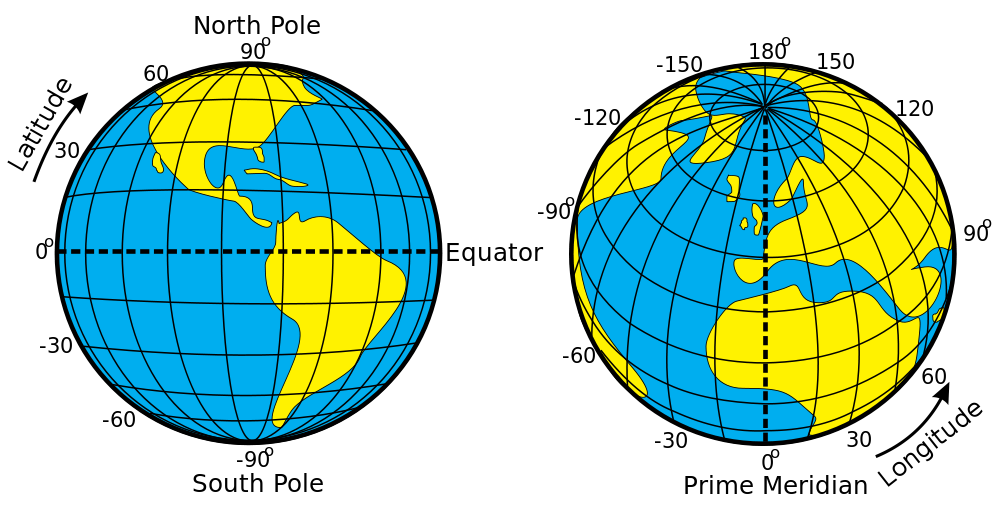
\includegraphics[height=2.5in]{figures/latitudelongitude.png}
    \caption[Latitude and longitude]{Illustration of Latitude $(\Phi)$ and Longitude $(\lambda)$. Obtained under the Creative Commons License from the Wikimedia Commons.}
\end{figure}

\subsection{Universal Transverse Mercator (UTM)}
\label{section:utm}

In order to describe the points on the Earth's surface in a two-dimension plane, as is desired for mapping, a projection model must be used on the angular latitude and longitude coordinates.  The projection model used in this research is known as the Universal Transverse Mercator (UTM) which splits the Earth into 60 lateral bands, examples of which are shown in figure \ref{utm_zones}.  In each zone an item is described by its easting, northing and altitude coordinates.  However, due to how the platform coordinate system is defined it's beneficial to have the Z axis in the downward direction.  This requires the easting and northing be switched to maintain a right-handed coordinate system. Therefore, UTM coordinates are described by $(N,E,D)$.  Another important modification is that the Z, or down, component is measured relative to the ground, not the WGS-84 ellipsoid. 

\begin{figure}[tbh]
	\centering
    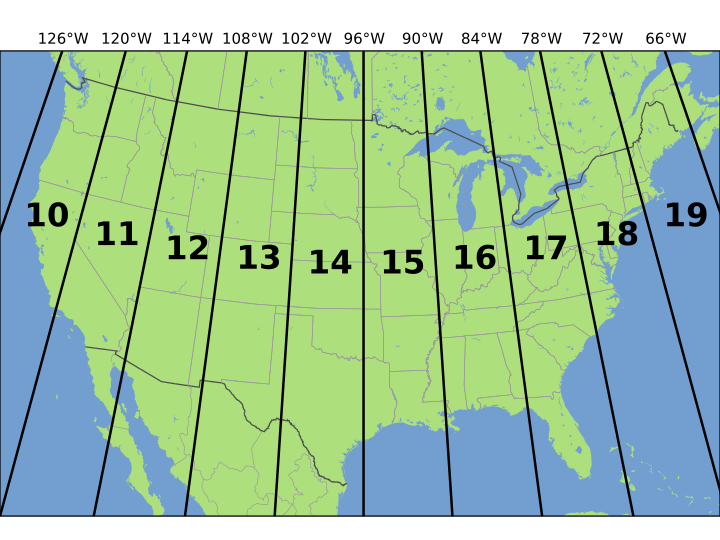
\includegraphics[height=2.5in]{figures/utm_zones.png}
    \caption[UTM zones]{Visualization of UTM zones over the United States. Obtained under the Creative Commons License from the Wikimedia Commons.}
    \label{utm_zones}
\end{figure}

\subsection{Field Coordinate System}

One issue with the easting and northing described by UTM is that rows in a fields are not always planted north and south or east and west.  Many of the post-processing steps benefit from removing this relative field orientation. A new field coordinate system is defined where the y-axis runs parallel to the rows and increases in the planting direction of the first row, and the x-axis increases in the direction of increasing row numbers.  The origin is selected so that all items in the field have positive x and y coordinates.   Similar to UTM the units of this frame are meters.  Coordinates in this frame are denoted $(x_f,y_f,z_f)$.

\begin{figure}[tbh]
	\centering
    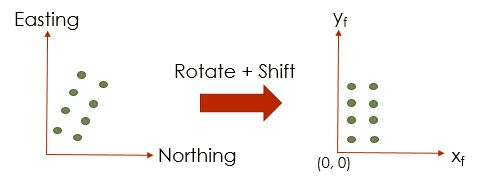
\includegraphics[height=2in]{figures/field_coordinates_small.png}
    \caption[Field coordinates]{Conversion from modified UTM coordinate frame (left) to field coordinate frame (right)}
    \label{field_coordinates}
\end{figure}

\subsection{Platform Coordinate System}
\label{platform_coordinate_system}

Another useful coordinate system is one fixed to the platform holding the cameras.  This coordinate system allows the relative spacing and orientation between the cameras and the GNSS <Todo already defined?> antenna to be specified.  Also this coordinate system defines how the platform's orientation is defined in terms of Euler angles, which is useful for accounting for non-level camera orientation.  The axes of this coordinate system are shown in the figure \ref{platform_frame}, which defines the x-axis out of the front of the platform, the y-axis out the right hand side and the z-axis orthogonal in the downward direction.  

\begin{figure}[tbh]
	\centering
    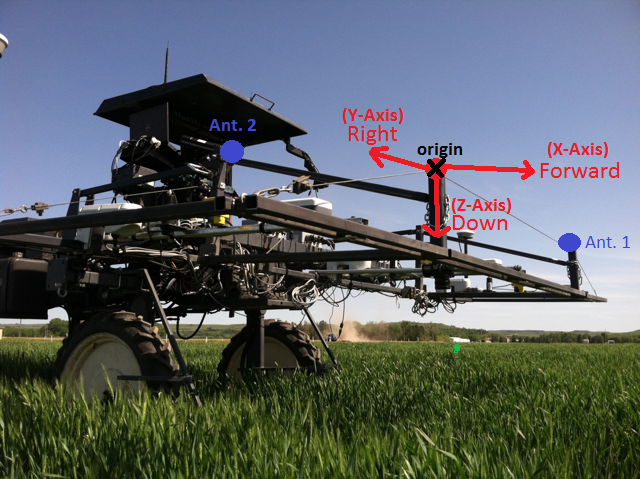
\includegraphics[height=4in]{figures/platform_frame_2_gps.png}
    \caption[Platform coordinate frame]{Example of platform coordinate frame on a tractor systems with two GNSS antennas shown in blue. The origin is the average of these antenna locations and is shown as a black X.}
    \label{platform_frame}
\end{figure}

\subsection{Camera Coordinate System}

The camera coordinate system describes the locations of objects in the world relative to the camera.  Typically a camera coordinate system is defined by the x-axis out of the right hand side of the camera, the y-axis out of the bottom and the z-axis along the optical axis.  <TODO cite>   However, for this application an alternative camera coordinate system is defined which has the x-axis out of the top of camera, the y-axis out of the right side and the z-axis along the optical axis.  This is so when the camera is mounted on the platform facing the ground with the top forward, the camera axes will align with the forward-right-down platform coordinate system.  This makes the meaning of the Euler angles consistent, and is also enforced by the data collection program.  The origin is defined to be located at a distance $f$ in front of the imaging sensor along the optical axis, where $f$ is the focal length of the lens.  This is discussed more in the next section.

\begin{figure}[tbh]
	\centering
    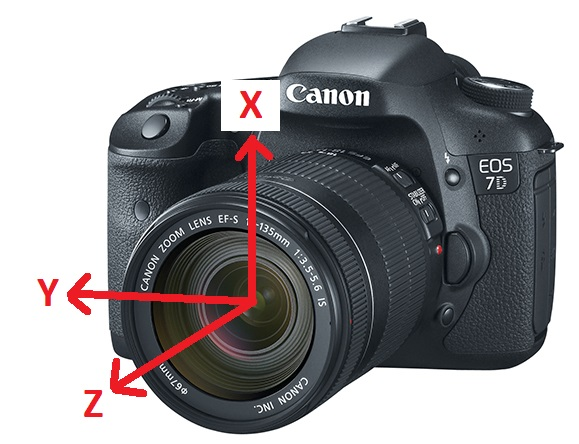
\includegraphics[height=2.5in]{figures/camera_frame_canon.jpg}
    \caption[Camera coordinate frame]{Image showing camera coordinate axes.}
    \label{platform_frame}
\end{figure}

\section{Coordinate Projections}
 
 An important step in the mapping process is converting between pixel and world coordinates, which is also the subject of many computer vision algorithms.  Since pixels are described in $\mathbb{R}^2$ and world points in $\mathbb{R}^3$, this conversion requires a projection.  
 
 However, before this can be defined a model must be chosen which describes how points in the world are projected onto the imaging sensor.  This section first presents the model used in this research and then discusses two equivalent methods that can be used for converting coordinates.  
 
 \subsection{Projection Model}
 
 A common choice for a thin, convex lens is the central perspective imaging model shown in figure \ref{projection_model}.
 
\begin{figure}[htb]
	\centering
    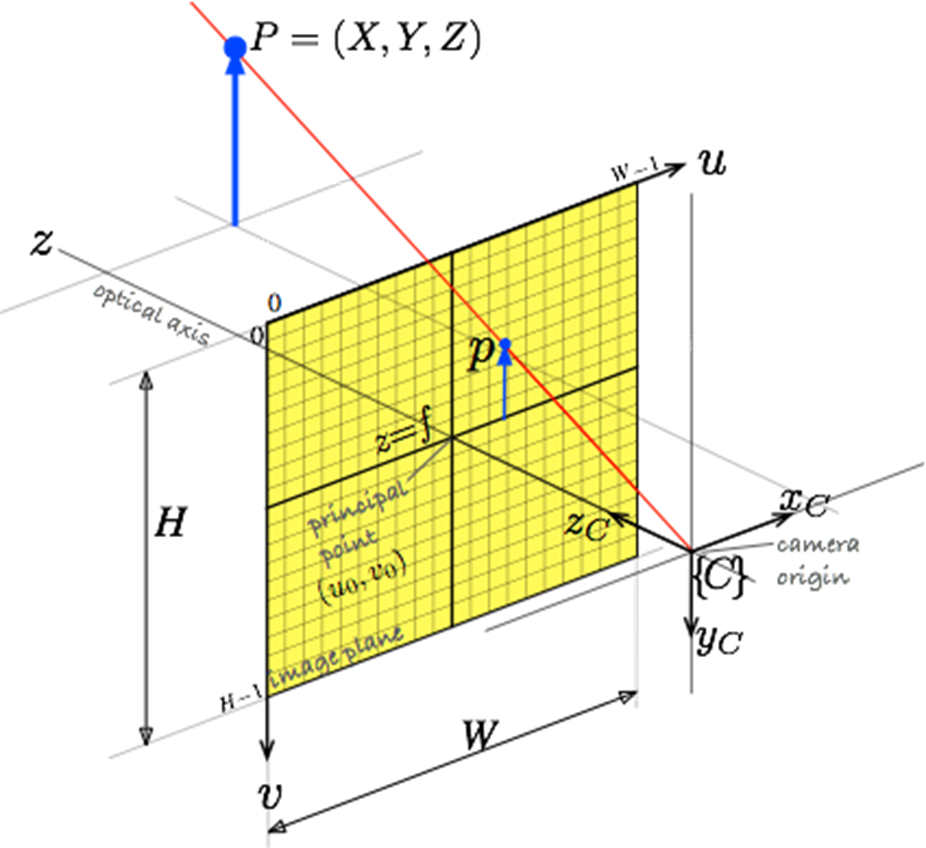
\includegraphics[height=4.5in]{figures/projection_model.png}
    \caption[Projection model]{Central perspective imaging model showing the image plane in yellow.  Adapted from "Robotics, Vision and Control" 1st edition, by Peter Coorke, 2013, p.252. Modified to show pixel frame in purple, the sensor frame in green and switched the ordering of the camera axes.}
    \label{projection_model}
\end{figure}
 
 This model is based on the concept of an ideal lens that is treated as an equivalent pin-hole, which implies the lens is perfectly focused and has no geometrical distortions.  The ideal lens will have two focal points along the optical axis which can be seen in figure \ref{focal_points}.  The central perspective model defines the image plane to be at the focal point in front of the lens, which is the left focal point shown in the figure.  

\begin{figure}[htb]
	\centering
    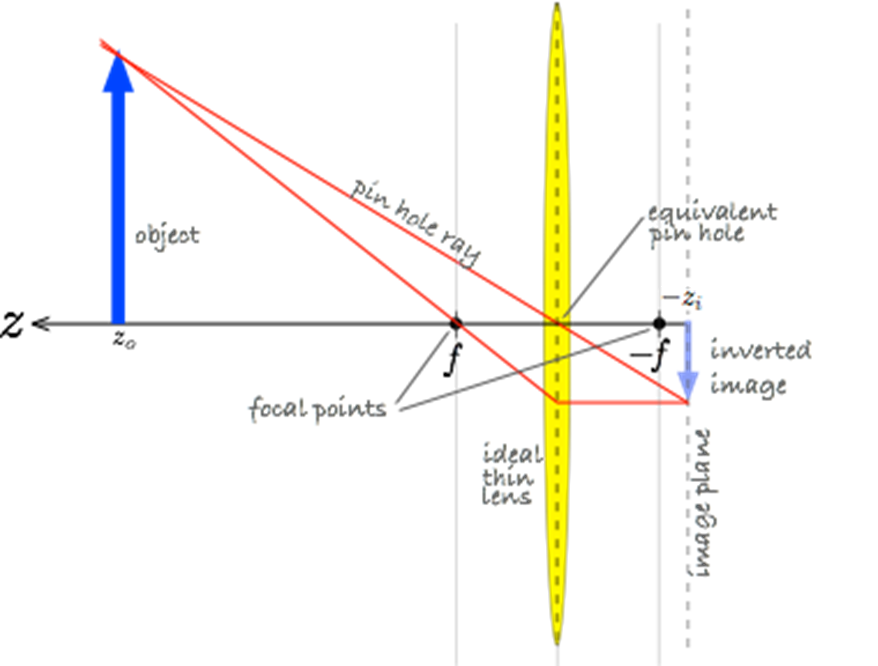
\includegraphics[height=2.5in]{figures/projections_two_focal.png}
    \caption[Focal points]{Equivalent pin hole lens showing both focal points. Adapted from "Robotics, Vision and Control" 1st edition, by Peter Coorke, 2013, p.252}
    \label{focal_points}
\end{figure} 

 Points in the image plane can be described using two different coordinate frames.  The first is the sensor frame and the second is the pixel frame.  The origin of the sensor frame is located at the point where the optical axis intersects the image plane.  A point in this frame is described by $(x,y)$, where the axes are in the same direction as camera frame and are shown in blue in figure \ref{projection_model}.  
 
 On the other hand, the origin of the pixel frame is located at the top left of the image plane and the x-axis increases to the right and the y-axis increases downwards.  Rather than $(x,y)$ a pixel's location is denoted as $(u,v)$.  The center of the image sensor is referred to as the principal point and is denoted $(u_0,v_0)$. Another key difference between these frames is the units.  The sensor frame has units of millimeters while the pixel frame has units of pixels.

 \subsection{Projection Methods}

 The conversion between pixel and world coordinates can go both ways, and both are used in the post-processing pipeline.  However, going from pixel to world coordinates is used more often and is slightly more challenging, so that is what is presented in this section. The conversion involves three frame transformations   
\begin{center}
 Pixel $(u,v)$ $\rightarrow$ Sensor $(x,y)$ $\rightarrow$ Camera $(X,Y,Z)$ $\rightarrow$ World $(N,E,DF)$
\end{center}
 
 This is referred to as a backwards projection, since it is projecting two-dimensional points back out into the world.  As mentioned above this is more challenging because depth information is lost during the forward projection as the image is captured.  There are many ways of recovering this depth information, which typically use multiple images or cameras.  However, the height of objects being mapped are relatively small and is not useful for this mapping application.  For that reason an assumption is made that every point in the world frame has a height of zero.  This reduces the world to a plane and results in a $\mathbb{R}^2$ to $\mathbb{R}^2$ mapping which is possible with a single image. 
 
 There are two different methods for performing this backwards projection. The first method discussed operates in Euclidean space and is more intuitive to understand.  The second method builds on this method by instead working in Projective space which produces a more efficient, but equivalent, conversion.  Both of these methods use the central perspective model and both make the same assumptions about the camera and lens.  These are:
 \begin{itemize}
 \item The lens does not cause any distortion. 
 \item There is no skew or displacement in how the image sensor is positioned within the camera.
 \item The focal length exactly matches the manufacturer's specification.
 \end{itemize}

 All of these assumptions are false to some extent, and it's possible to correct these assumptions using certain camera calibration procedures <TODO cite>.  However, for the system presented in this research these effects are considered negligible.  Another assumption is the camera's orientation is relative to the ground.  However, typically orientation angles are measured with respect to the gravity vector, which on hills will not be orthogonal to the ground.  If the mapping is done on a hill then the simplest solution is to make sure the camera's orientation about the platform's X and Y axes is zero.
 
 \subsubsection{Euclidean Space}
 
 The first transformation is to convert pixel coordinates to sensor coordinates.  Using the frame definitions shown in figure \ref{projection_model}, this can be represented in matrix form as 
 
\[
\begin{bmatrix} x \\ y \end{bmatrix}
=
\begin{bmatrix} 
 0 & -\rho_h \\
 \rho_w & 0 
\end{bmatrix}
\begin{bmatrix} u \\ v \end{bmatrix}
+
\begin{bmatrix} \rho_h v_0 \\ \rho_w u_0 \end{bmatrix}
\]
 
 where $\rho_w$ and $\rho_h$ are the width and height of each pixel in millimeters, and $u_0$ and $v_0$ are the coordinates of the principal point in pixels.   The next transformation is to convert from sensor coordinates to camera coordinates.  It's clear from the projection model that if the sensor coordinates are combined with the focal length $f$ as
 \begin{center}
 $(x,y,f)$
 \end{center}
 then the result is a vector in the camera frame, but with units of millimeters rather than meters. The last frame transformation is to describe this vector in terms of the world frame.  This can be accomplished by a rotation matrix $R$
 
 \begin{equation}
 \label{rotation_eq}
 \begin{bmatrix} n \\ e \\ d \end{bmatrix}
 =
 R *
 \begin{bmatrix} x \\ y \\ f \end{bmatrix}
 \end{equation}

 where this rotation matrix is composed from the active, extrinsic rotations about the worlds north, east and down axes in that order, by angles $\phi$ (roll), $\theta$ (pitch) and $\psi$ (yaw).  These are the Tait-Bryan angles of the camera frame with respect to the world frame.  Technically this is a passive rotation by negative angles since the vector is changing frames, but using active rotations avoids many double negatives.
 
  \begin{align}
  \label{rotation_equation}
  R &= R_z(\psi)*R_y(\theta)*R_x(\phi) \\ \notag
    &= \begin{bmatrix} \cos(\psi)  & -\sin(\psi) & 0 \\ 
                        \sin(\psi) & \cos(\psi) & 0 \\
                         0         &   0         & 1  \end{bmatrix} 
       \begin{bmatrix} \cos(\theta) & 0 & \sin(\theta) \\ 
                             0      & 1 &       0        \\
                      -\sin(\theta) & 0 & cos(\theta) \end{bmatrix}
       \begin{bmatrix} \ 1 &    0       & 0           \\ 
                         0 & \cos(\phi) & -\sin(\phi) \\
                         0 & \sin(\phi) & cos(\phi)  \end{bmatrix} \\ \notag
    &= \begin{bmatrix} \cos(\theta)\cos(\psi) & \sin(\phi)\sin(\theta)\cos(\psi) - \cos(\phi)\sin(\psi) &  \sin(\phi)\sin(\psi) +  \cos(\phi)\sin(\theta)\cos(\psi) \\
    \cos(\theta)\sin(\psi) & \cos(\phi)\cos(\psi) + \sin(\phi)\sin(\theta)\sin(\psi) &  \cos(\phi)\sin(\theta)\sin(\psi) - \sin(\phi)\cos(\psi) \\
     -\sin(\theta) & \sin(\phi)\cos(\theta) & \cos(\phi)\cos(\theta)     \end{bmatrix}
  \end{align}
  
 Lowercase coordinates $(n,e,d)$ in equation \ref{rotation_eq} are used to designate that these components are in the north, east and down directions, but the units are still in millimeters and this does not represent the world point yet.  The position of this vector in the world frame is given by the camera's world position

 \begin{equation}
 \label{translation_equation}
 T = 
 \begin{bmatrix} T_x \\ T_y \\ T_z \end{bmatrix} =
 \begin{bmatrix} N_{cam} \\ E_{cam} \\ D_{cam} \end{bmatrix}
 \end{equation}

 The actual world point can be found by finding the intersection of this vector, $(n,e,d)$, with the flat plane of the Earth given by the equation $D=0$.  
 
 This can be done by parameterizing the vector with $S$ as 
 
 \begin{equation}
 \label{parameter_ned}
 \begin{bmatrix} N \\ E \\ D \end{bmatrix} =
 S \begin{bmatrix} n \\ e \\ d \end{bmatrix}
 + \begin{bmatrix} T_x \\ T_y \\ T_z \end{bmatrix}
 \end{equation}
 
 plugging in the third component, $D$, into the plane equation and solving for
 \begin{center}
 $S = -T_z / d$, 
 \end{center}
 which can be plugged back into equation \ref{parameter_ned}.  If $d$ is zero then the position vector is parallel to the Earth's surface and will never intersect it.   

 While this method is easy to visualize, it requires multiple steps for each pixel that must be converted to world coordinates.  A more efficient method is presented in the next section.

 \subsubsection{Projective Space}
 \label{section:projection_space}
 
 An ideal solution would be to describe the backwards projection from the pixel plane to the world plane as a single matrix that can be applied in one step.  In order to do this, coordinates in each frame must be converted into the Projective space which adds an extra coordinate.  This coordinate represents scale, and a set of coordinates in this space is referred to as homogeneous coordinates.

 There are many benefits to using homogeneous coordinates which is why they are commonly used in computer vision.  These benefits include
 \begin{enumerate}
 \item performing translations and rotations in a single matrix.
 \item avoiding unnecessary division in intermediate calculations which is typically slower than other operations.
 \item representing a coordinate at infinity with real numbers which is true when the extra coordinate is zero.
 \end{enumerate}
 
 In order to differentiate between regular Euclidean coordinates, homogeneous coordinates are followed by an apostrophe.  For example coordinates in the pixel frame can be described in Projective space as $(u',v',w')$ where 
 
 \begin{center}
 $u' = u*w'$ and $v'=v*w'$.
 \end{center}
 
 In backwards projection the pixel coordinates $(u,v)$ are what is known so $w'$ is always set to 1 so it does not change the scale.   In order to convert from pixel to sensor coordinates the same relationship using the pixel sizes and principal point are used, however when homogeneous coordinates are substituted this relationship can be described in a single matrix
 
 \[
 \begin{bmatrix} x' \\ y' \\ z' \end{bmatrix}
 =
 \begin{bmatrix} 
     0   & -\rho_h & \rho_h v_0 \\ 
  \rho_w &    0    & \rho_w u_0 \\
     0   &    0    &      1  
 \end{bmatrix}
 \begin{bmatrix} u' \\ v' \\ 1 \end{bmatrix}
 \]
 
 This is typically referred to as the inverse parameter matrix, or $K^{-1}$.  The second transformation is to convert sensor coordinates to camera coordinates.  A consequence of defining the origin of the camera frame to be the location of the equivalent pin-hole is that all incoming rays of light converge to the origin of the camera frame.  This leads to the simple relationship using the focal length $f$ of
  
  \begin{center}
  $x=fX/Z$  and $y=fY/Z$
  \end{center}
 
  which can easily be derived by similar triangles.  When described as homogeneous coordinates this relationship becomes 
  
  \begin{center}
  $x'=fX$, $y'=fY$ and $z'=Z$
  \end{center}
  
  or in matrix form
  
   \[
   \begin{bmatrix} X_u \\ Y_u \\ Z_u \end{bmatrix}
   =
   \begin{bmatrix} 
       1/f &   0   &  0 \\ 
       0   &  1/f  &  0 \\
       0   &   0   &  1  
   \end{bmatrix}
   \begin{bmatrix} x' \\ y' \\ z' \end{bmatrix}
   .
   \]
   
  The subscript $u$ denotes that these coordinates in the camera frame are unscaled, similar to how $(x,y,f)$ is not correctly scaled in the Euclidean method.  Also note that $(X_u, Y_u, Z_u)$ are not homogeneous coordinates.  This matrix is referred to as the inverse camera matrix, or $C^{-1}$.   The last frame transformation is to go from the camera to world frame and correctly scale the position vector.  This can be done in one step if homogeneous world coordinates $(N',E',D',S')$ are used.  In terms of the rotation matrix $R$ and translation vector $T$ defined in equations \ref{rotation_equation} and \ref{translation_equation}  
  
     \[
     \begin{bmatrix} R^{-1} & -T \end{bmatrix}
     \begin{bmatrix} N' \\ E' \\ D' \\ S' \end{bmatrix}
     =
     \begin{bmatrix} X_u \\ Y_u \\ Z_u \end{bmatrix}
     .
     \]
     
 If each element in $R$ is denoted by its row, $i$, and column, $j$, as $R_{ij}$, and since the inverse of an orthogonal matrix is equal to its transpose then this is expanded to
 
      \[
      \begin{bmatrix} r_{11} & r_{21} & r_{31} & -T_x \\
                      r_{12} & r_{22} & r_{32} & -T_y \\
                      r_{13} & r_{23} & r_{33} & -T_z \\
      \end{bmatrix}
      \begin{bmatrix} N' \\ E' \\ D' \\ S' \end{bmatrix}
      =
      \begin{bmatrix} X_u \\ Y_u \\ Z_u \end{bmatrix}
      .
      \]
      
  However, this matrix is clearly not invertible and the assumption that $D=0$ must be enforced.  Since $D'=D/S'$ then $D'$ is also zero, and it can be removed along with the third column of the matrix.   After inverting this results in 
  
  \[
    \tilde{p} =
    \begin{bmatrix} N' \\ E' \\ S' \end{bmatrix}
      = 
    \begin{bmatrix} r_{11} & r_{21} & -T_x \\
                    r_{12} & r_{22} & -T_y \\
                    r_{13} & r_{23} & -T_z \\
    \end{bmatrix}^{-1}
    \begin{bmatrix} X_u \\ Y_u \\ Z_u \end{bmatrix}
  .
  \]
 
  Even though an entire column of the rotation matrix is discarded no information is lost as this column can be described as the cross product of the first and second columns.  This inverted matrix is denoted $\xi^{-1}$, so that the entire projection can be represented as a single homography matrix
  
 \begin{equation}
 H = \xi^{-1} C^{-1} K^{-1} 
 \label{equation:homography}
 \end{equation}
 
 Once $(N',E',S')$ is computed the actual northing and easting is simply the inhomogeneous coordinates
 
 \begin{center}
 $N=N'/S'$ and $E=E'/S'$
 \end{center}
 
 While it's not obvious, this result is indeed equivalent to the one derived in the first method.  This is verified symbolically in Appendix {TODO ref}.  


\cleardoublepage

\chapter{System Design}
\label{chapter:system_design}

The mapping system consists of the various components needed to capture, organize and locate images of the field, as well as any additional field items needed for identifying plants.  The proper design of the mapping system is the most important step in the overall mapping process.  Poor design leads to insufficient image quality, missing field coverage or improperly located images, which no amount of post-processing can correct.  

The first part of the system discussed is the markers used for plant identification because the required size of these markers impose constraints on the rest of the system.  Next, the base platform and additional equipment, such as cameras, is presented along with reasoning about nominal parameters such as vehicle speed and the camera height above the ground.  This chapter concludes by describing additional field markers which are not strictly necessary, but help improve the robustness of the mapping process. 

\section{Plant Identification}
\label{section:plantid}

As mentioned in the introduction chapter, the mapping process involves not just determining plant coordinates, but also assigning each plant to a group.  Each plant group is referenced by a unique identifier (ID), such as 1035.  The method used in this research is to encode this ID in a two-dimensional barcode that is placed at the beginning of each group of plants in the field. 

If a plant group needs to be planted in different parts of the field then a repetition letter is appended to the group number.  For example, three codes containing the text 1035A, 1035B and 1035C all belong to plant group 1035.  Since the two-dimensional barcodes are only placed at the beginning of the group it's critical to know the direction each row is planted in order to associate the correct set of plants with the plant ID.  Codes could be placed on both sides of each group to remove this added challenge, but this doubles the amount of code construction time, field debris and chance of missing a code during the post-processing.  Instead the row direction is encoded in row markers which is discussed later in this chapter.

\subsection{Code Format}
\label{section:code_format}

For this research project, Quick Response (QR) codes were selected as the barcode format. This is a standardized format that was made publicly available by Denso Corporation over 20 years ago.  It was first used for item tracking in the Japanese automotive industry, and has most recently become well known for encoding Uniform Resource Locators (URLs) for websites. <TODO ref article>.  Two important characteristics of this format is it can be read from any orientation, and it can still be read if part of the code is damaged.  Various other types of formats, such as Aztec or Micro QR, can encode information in smaller grids by restricting the character encoding, but offer less error correction.  Also, at the time this research was conducted these alternate formats were not supported by any of the open-source readers that the researcher investigated. 

\begin{figure}[htb]
	\centering
    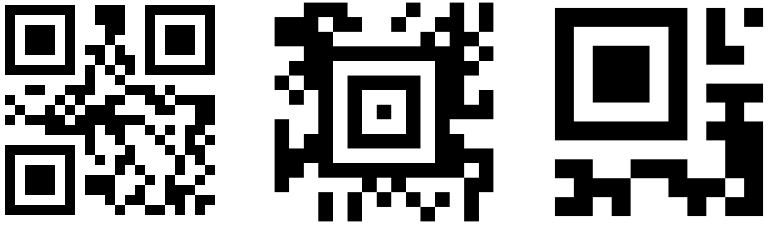
\includegraphics[width=3in]{figures/generated_codes_1035.png}
    \caption[2D barcode formats]{Comparison of 2D barcode formats encoding the text 1035 with high error correction.  From left to right: Quick Response (QR), Aztec and Micro QR.}
    \label{barcode_formats}
\end{figure} 

\subsection{Size Constraint}

For fields with thousands of different plant groups it's not feasible to place these QR codes by hand.  Therefore, they must fit through the deposit cylinders of the transplanter shown in figure \ref{figure:transplanter}.  In order to not get caught in the cylinders the codes cannot be larger than 2.5 centimeters in diameter. Since there needs to be a white margin around the actual QR code, the code itself ends up being roughly 2 centimeters.  The QR code format is split into different versions which define how many squares make up the code.  The first version is a grid of 21 by 21 squares and is shown in figure \ref{barcode_formats}.  This results in a maximum square size of only 1 millimeter.  

\subsection{Code Construction}

The codes must be easy to produce due to the potentially large number of codes required for each field.  The <TODO> program can be used to generate all QR codes at once, and a thermal printer can print the codes on pot labels rapidly.  However, the pot labels need a solid base to stay upright and grounded during transplanting. The researchers at the Land Institute in Salina, Kansas, developed a biodegradable base <TODO better describe base> that the pot labels are inserted into.  An example of one of these QR codes can be seen in figure \ref{QR_code}.

\begin{figure}[htb]
	\centering
    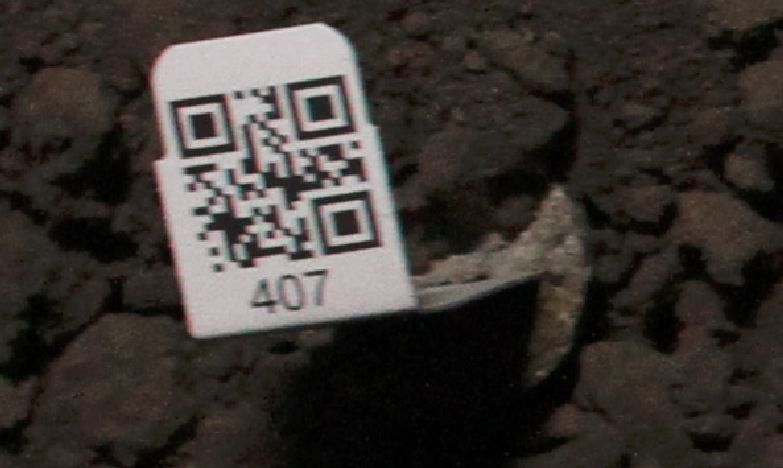
\includegraphics[height=2in]{figures/qr_code_407.png}
    \caption[QR code]{QR code printed on pot label and planted in field.}
    \label{QR_code}
\end{figure}

\section{Platform Design}
\label{section:platform_design}

There are many types of platforms that could be used for mapping.  Aerial vehicles have the benefit of autonomously traversing the field without the possibility of running over plants. However, they are unable to provide external lighting or shading which is important when post-processing the images. In addition, the size constraint on QR codes would require low altitude flights at a constant altitude to keep the codes properly focused, which is not easy to achieve.  Higher altitude flights would be possible with a telescopic lens, but this increases cost, weight and most critically the effects of error in camera orientation.  For these reasons only ground platforms are considered.

Two different types of ground platforms are investigated, a manual push-cart and a four-wheel robotic vehicle.  The push-cart excels in it's simplicity, however for this thesis only the robotic platform is discussed.  The main benefits of a robot is the ability to drive at a constant speed and the option to operate autonomously.  Driving at a constant speed is important to ensure sufficient overlap between successive images, and self-driving vehicles remove much of the tedious work associated with imaging large fields.  

\subsection{Robotic Platform}

The selected robotic platform is the Husky A2000 mobile robot made by Clearpath Robotics.  The Husky is a four wheeled differential drive robot measuring 39 inches in length and 27 inches wide.  It features a maximum speed of 1 meters per second and can carry up to 75 kilograms.  A custom C-channel structure was added to the top of the robot to enable it to image the field.  This structure can be seen in figure \ref{husky_rocky_ford}.  Attached to the front of the structure are two Canon 7D digital single-lens reflex (DSLR) cameras.  Using two cameras allows two rows to be mapped at the same time. 

\begin{figure}[htb]
	\centering
    \includegraphics[height=2.7in]{figures/sunflower_rocky_ford_labeled.jpg}
    \caption[Husky]{Husky mobile robot equipped with two cameras.}
    \label{husky_rocky_ford}
\end{figure}

On the back of the C-structure are two white Trimble AG25 antennas, which attach to a Trimble BX982 global navigation satellite system (GNSS) receiver.  This receiver is mounted to the top of the robot.   

\subsection{GNSS Receiver}

The BX982 receiver provides centimeter level accuracy when paired with a fixed base receiver broadcasting RTK correction signals.  For this application the fixed base is a Trimble Ag542 receiver with a Trimble Zypher Geodetic antenna as shown in figure \ref{base_station}.  This base station communicates with the SNB900 rover radio mounted on the robot over a 900 MHz radio link.   The dual antenna design allows the robot to determine its heading, or yaw, to within approximately 0.1 degree.  This accurate yaw is important for geo-locating plants and QR codes within images, as well as allowing the robot to operate autonomously as discussed in section \ref{section:automated_control}. 

\begin{figure}[htb]
	\centering
    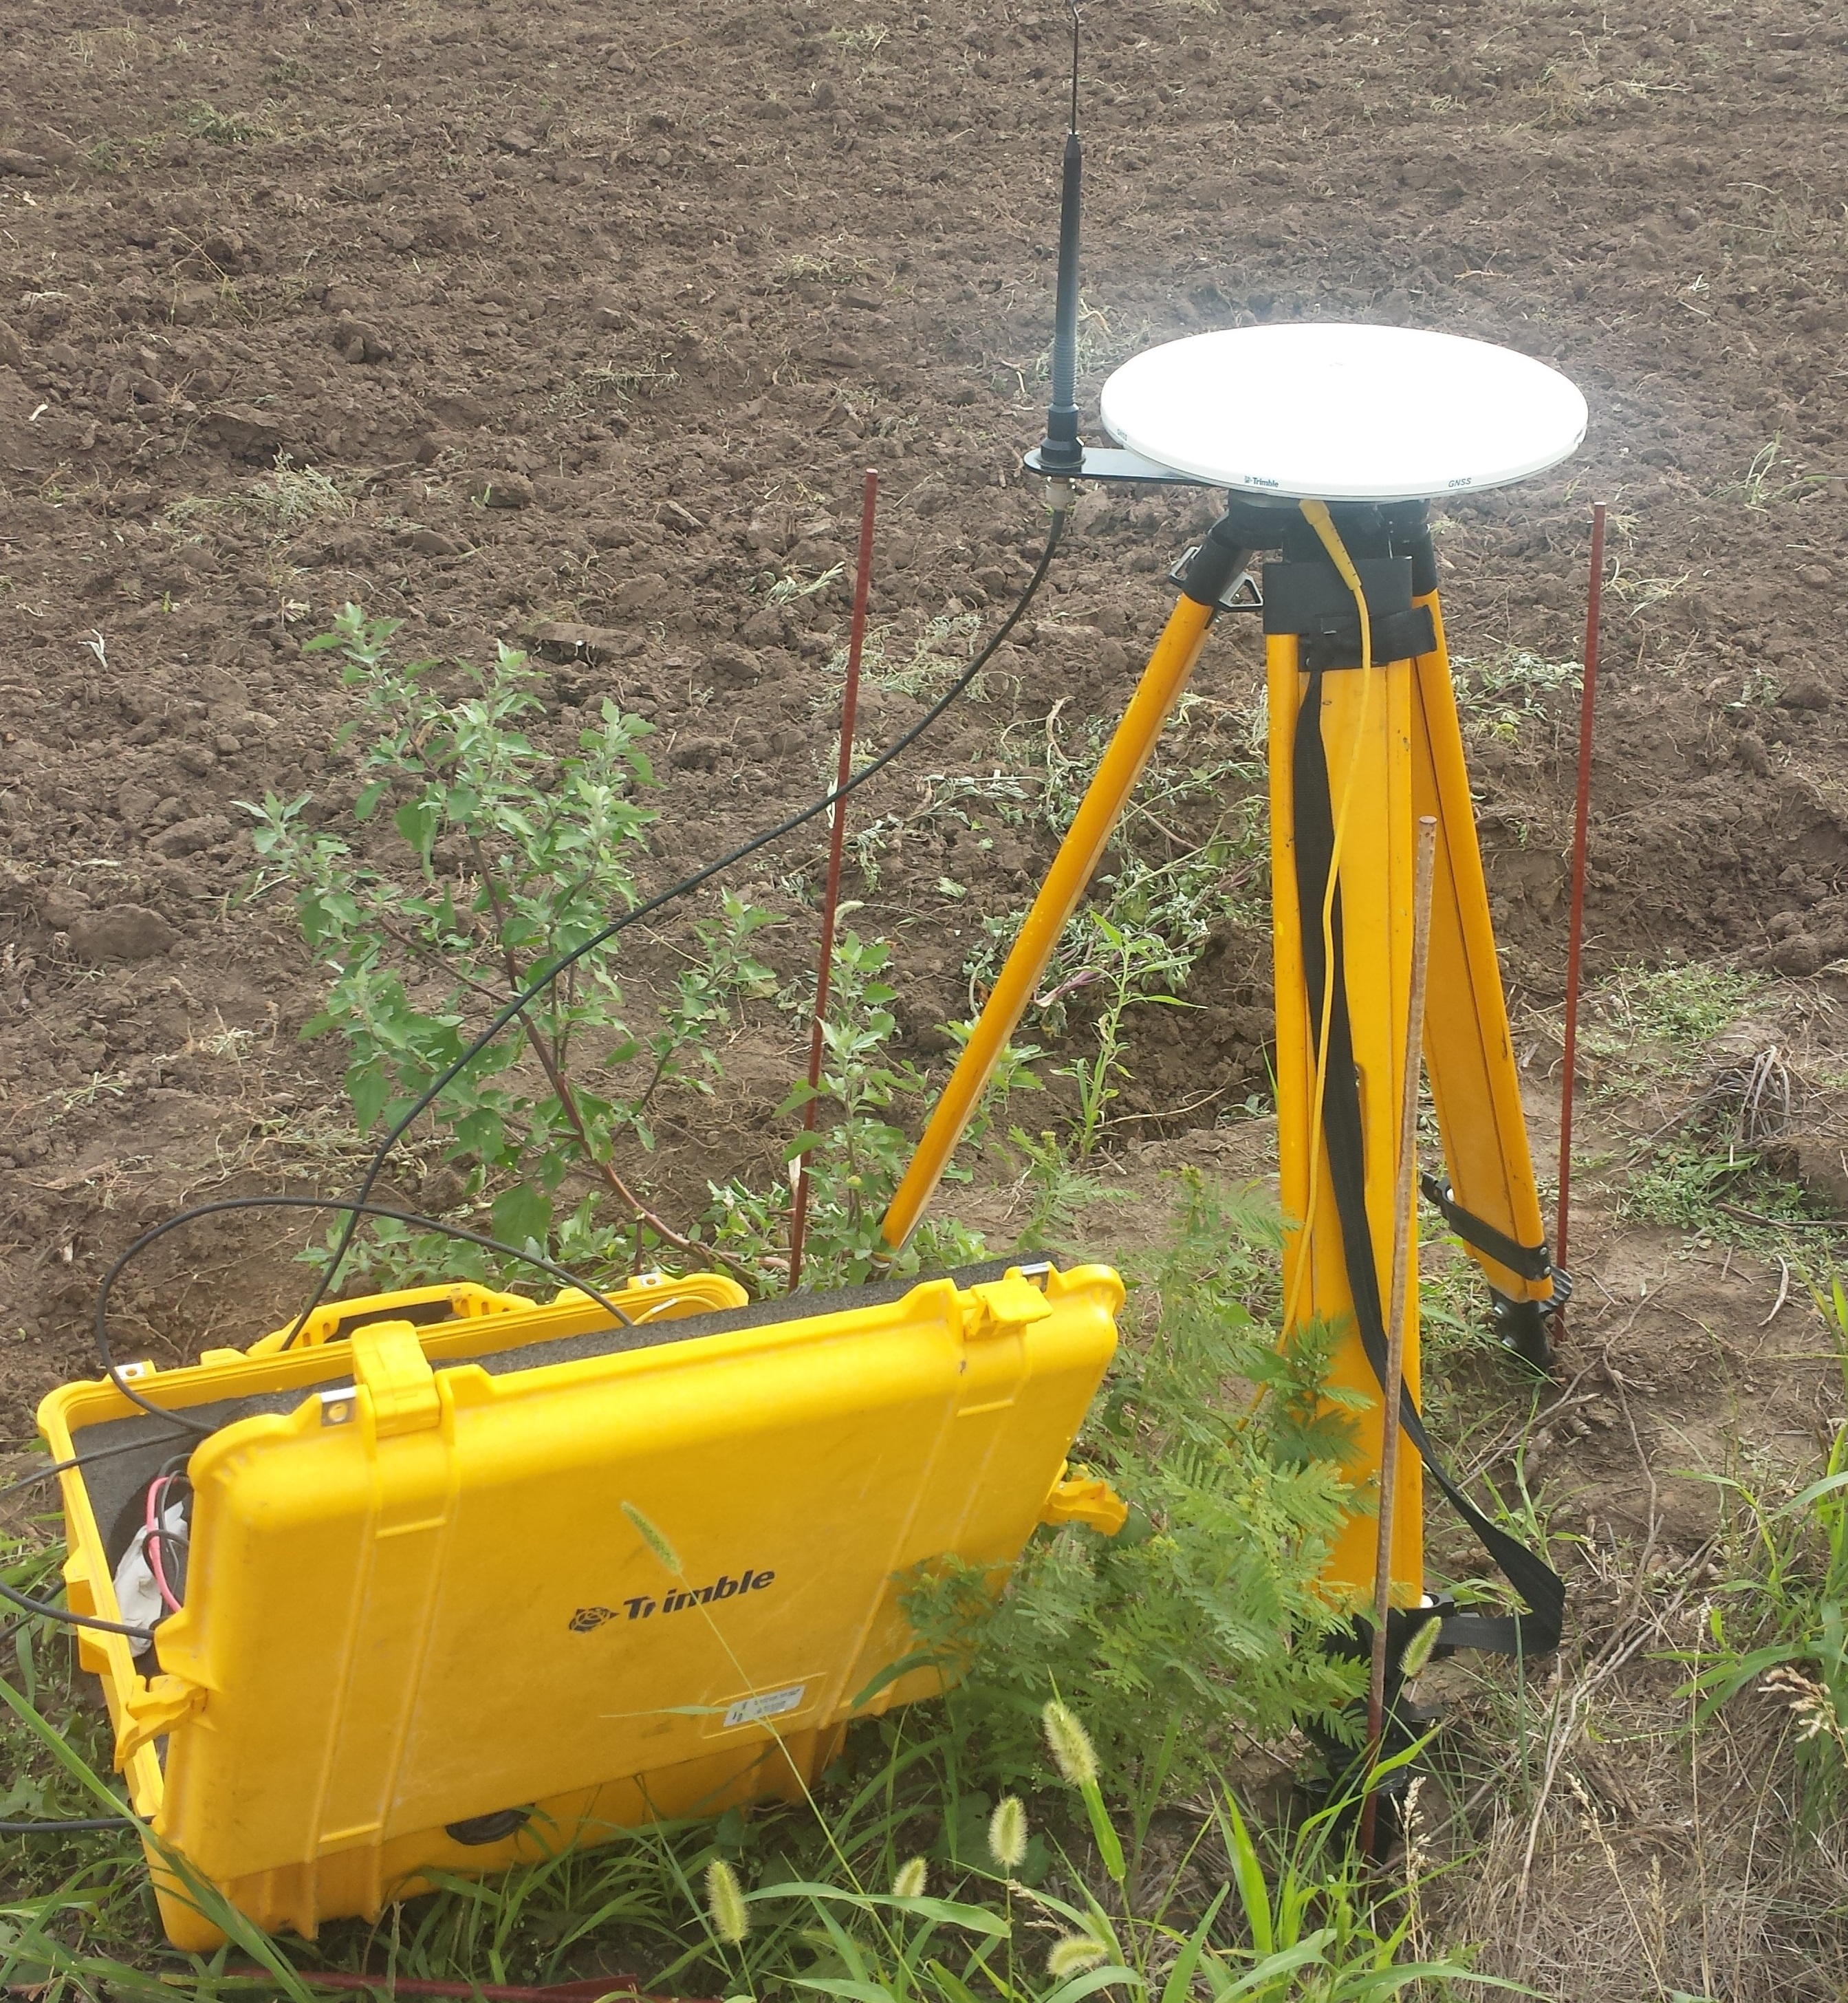
\includegraphics[height=3in]{figures/sunflower_base_cropped.jpg}
    \caption[Base station with tripod]{Ag542 base station mounted on tripod.}
    \label{base_station}
\end{figure}

\subsection{Cameras and Lighting}

The Canon 7D features an 18 megapixel (MP) sensor and is fitted with a fixed 20 millimeter focal length wide-angle lens.  The camera contains an Advanced Photo System type-C (APS-C) sensor rather than a full frame 35mm sensor. When paired with the wide-angle lens this gives a horizontal angle of view of 58.3 degrees and a vertical view of 40.9 degrees.  
As shown in figure \ref{husky_rocky_ford} the cameras are mounted far out in front of the robot so that the wheels and front bumper do not show up in the image and effectively reduce the field of view.  In addition, each camera is mounted with a 90 degrees yaw offset with respect to the platform so that the longer side of the image is aligned with the forward movement of the robot as seen in figure \ref{figure:image_fov}.  

\begin{figure}[htb]
	\centering
    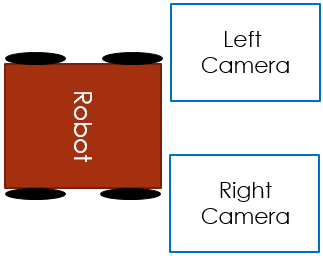
\includegraphics[height=2in]{figures/camera_directions.png}
    \caption[Camera field of view]{Depiction of camera field of views relative to robotic platform.}
    \label{figure:image_fov}
\end{figure}

An item that is not pictured on the robot, but is shown in figure \ref{figure:canon_and_bars} is a light emitting diode (LED) bar.  These 9 watt bars provide external lighting at night time for consistent image lumination.  It is feasible to only use 2 bars, one for each camera, however using 4 bars provides enough light for the camera settings to be set conservatively.  Another benefit of using one bar on each side of each camera is it noticeably reduces image glare on the QR codes.  

\begin{figure}[htb]
	\centering
    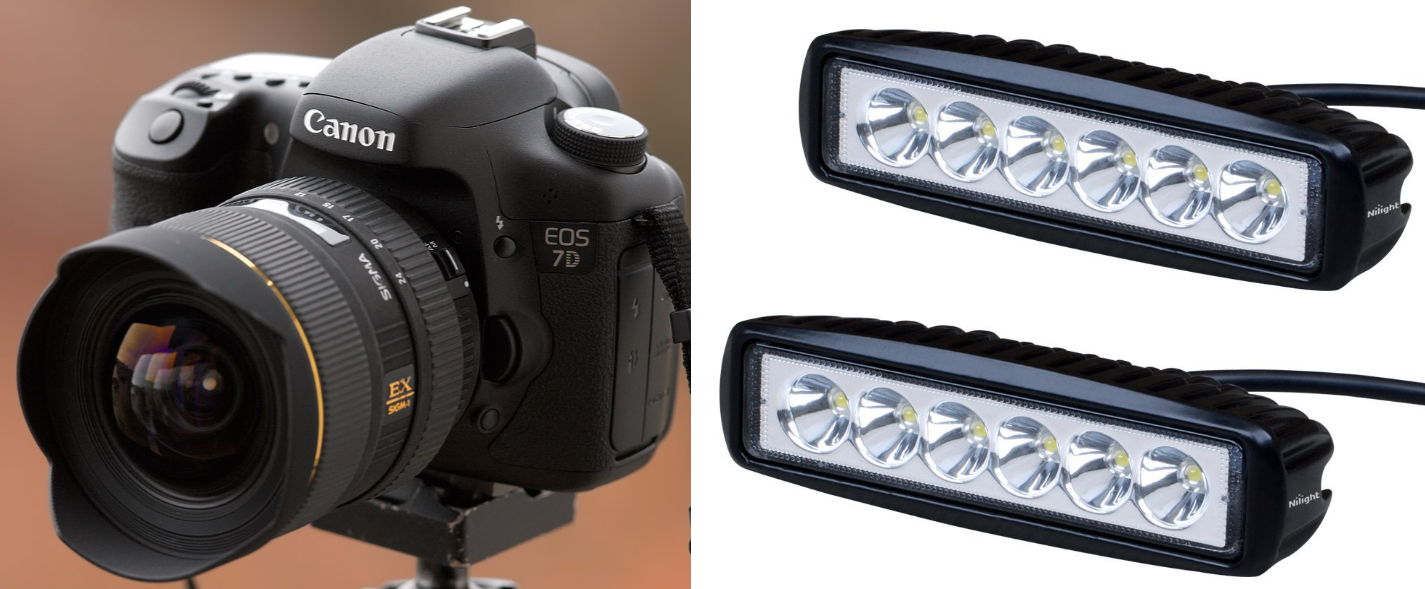
\includegraphics[height=2in]{figures/canon7d_and_LEDs.png}
    \caption[Canon 7D and LED bars]{Canon 7D and external lighting bars.}
    \label{figure:canon_and_bars}
\end{figure}

\subsection{Determining Parameters}
\label{section:determining_parameters}

There are many parameters, such as camera height and vehicle speed, which are chosen to ensure quality images and sufficient field coverage.  The most important to determine first is the camera height, as that determines the resolution of the image.  If the image resolution is too low then the QR codes will be unreadable.  
If each pixel could correspond to exactly one square on the QR code then the minimum resolution would be 1 pixel per millimeter, since each square is roughly 1 millimeter in size.  In reality this is almost never the case, and the theoretical minimum is 3 pixels for one square.  If only 2 pixels per square are used then the light from the square could be split in half with the adjacent white square and the result would be an unresolved gray square.  However, all lenses also introduce some loss in contrast.  The amount of contrast lost is a function of many things such as lens diffraction, aperture and pixel position.  Also in reality the camera's optical axis is not always perfectly orthogonal to the QR code.  To account for these extra effects the actual minimum resolution is set to 5 pixels per millimeter.  

The 18 million effective pixels on the sensor are split into a 5184 by 3456 grid.  The minimum resolution then requires a maximum image size of 1037 by 690 millimeters, which constrains the cameras to be no higher than 930 millimeters above the QR codes.  In order to make the imaging process more robust, the cameras are mounted 700 millimeters above the ground which corresponds to an image size of 781 by 520 millimeters, and a resolution of approximately 6.5 pixels per millimeter.  Mounting the cameras lower than the maximum requirement also always the external lighting to be more concentrated and requires smaller shading if the imaging is done during the day.  

Another requirement that is added to make the mapping process more robust is each QR code must be in a minimum of two images.  This helps solve temporary issues such as bugs flying in front of the camera as well as offers multiple perspectives if the code is accidentally planted at an angle.  In order to ensure this the maximum spacing between successive images is given by the equation
\begin{align*}
 \text{max spacing} &= (\text{image width} - \text{QR side length} - \text{pad}) / 2 \\
             &= (781 - 25 - 75) / 2 \\ 
             &= 340 \text{ millimeters}
\end{align*}
where the pad is extra spacing to account for variations in camera latency and reduced lighting at the image border.
  
An additional constraint on the cameras that must be taken into account is the minimum trigger period.  Many cameras, including the Canon 7D, are capable of exposing images rapidly and then buffering them before they are processed.  However, the minimum trigger period considered in this section is the minimum amount of time for an image to be exposed, processed and saved without continued buffering, as buffering can only be sustained for so long.  This was experimentally determined for the Canon 7D to be 0.7 seconds.  

In order to satisfy the maximum image spacing, while not exceeding the minimum trigger period, the robot cannot drive faster than 0.5 meters per second.  One downside of driving this fast is cameras begin to noticeably shake when the field is not smooth, which can lead to blurry images.  Therefore the nominal robot speed is set to 0.4 meters per second.  These platform parameters are summarized in table \ref{table:platform_params}.

\begin{table}[htb]
    \begin{center}
    \caption{Summary of platform parameters.}
    \begin{tabular}[c]{|c|c|c|}
        \hline
        Parameter & Value & Units \\
        \hline
        Camera Height    & 700       & millimeters         \\
        Image Size       & 781 x 520 & millimeters         \\
        Image Resolution & 6.5       & pixels / millimeter \\
        Trigger Period   & 0.7       & seconds / image     \\
        Robot Speed      & 0.4       & meters / second     \\
        \hline
    \end{tabular}
    \label{table:platform_params}
   \end{center}
\end{table}

\subsection{On-board Computers}

There are a total of four computers used on the Husky.

\begin{description}
\item[Main Husky Computer] - custom mini-ITX situated inside the main compartment of the robot running Ubuntu 12.04 along with the Robot Operating System (ROS). This computer contains all of the telemetry and guidance logic and is discussed more in section \ref{section:base_functionality}.  
\item[Husky Microcontroller] - Atmel ARM-based SAM7XC256 enclosed in the back of the robot chassis.  This microcontroller receives linear and angular velocity commands from the main computer and reports feedback from the robot's encoders, battery and motors. 
\item[Husky Interface Computer] - Lenovo T400 laptop that is also running Ubuntu 12.04 along with ROS.  This computer sits on top of the Husky and is used to send commands to the robot using a secure shell (SSH)
\item[Data Collection Computer] - Lenevo S431 laptop running Windows 7 that also sits on top of the Husky.  This computer runs the program responsible for saving data from the cameras and GNSS receiver.   
\end{description}

For simplicity the output of the GNSS receiver is split to both the data collection computer as well as the main Husky computer.  It would be ideal to run the data collection program on the Husky interface computer to eliminate the need for an extra computer.  However, the data collection program requires a Windows based operating system to interact with the Canon cameras, and at the time of this research ROS is not stable on Windows. 

\section{Guidance and Control}

The Husky arrived from Clearpath with basic driving functionality, however this was not sufficient for the mapping process.  This section describes the additional functionality developed for the robot that enables it to operate in autonomous or semi-autonomous modes.  

\subsection{Base Functionality}
\label{section:base_functionality}

When the Husky was purchased the main computer came installed with the Robot Operating System, which is popular open-source framework that provides many of the same services as traditional operating system such as inter-process communication and hardware-abstraction.  One major benefit is ROS allows different functionality to be split up into separate processes, referred to as nodes.  This promotes code re-use and prevents one component from crashing the entire system.   The nodes that were pre-installed on the Husky are listed below.

\begin{description}
\item[Teleop node] - receives driving commands from the Logitech controller shown in \ref{figure:cruise_control}.  The default functionality is when the X button is held down and the left and right analog sticks command linear and angular velocity, respectively.
\item[Husky node] - in charge of sending the velocity commands over a serial port to the microcontroller that controls the motors.  
\item[IMU node] - driver for the UM6 orientation sensor that came installed on the robot.  However, this node is not used since the platform is stable and the multiple GNSS antennas determine yaw.
\end{description}

\subsection{Cruise Control}

When driving through the field it's important that the robot maintains a constant speed to ensure all QR codes and plants are imaged.  With the basic teleop functionality this was difficult to achieve while also keeping the robot centered in the middle of the row. To solve this issue the researcher extended the teleop node to include cruise control functionality that is commonly seen in automobiles.  

\begin{figure}[htb]
	\centering
    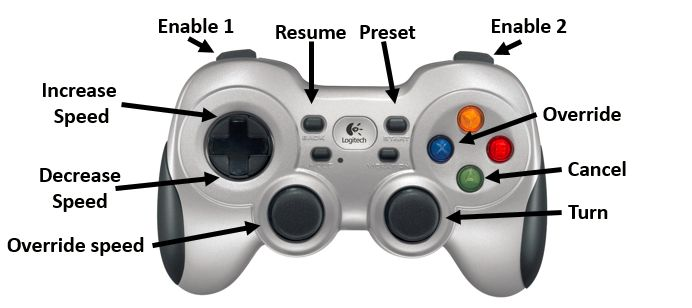
\includegraphics[height=3in]{figures/logitech_controller_labelled.png}
    \caption[Cruise control buttons]{Logitech controller for Husky showing cruise control functionality.}
    \label{figure:cruise_control}
\end{figure}

Cruise control can be enabled by either pressing both the Enable 1 and Enable 2 buttons at the same time or by the Preset button.  The Preset button defaults to a certain configuration speed, by default 0.4 meters per second.  If the Override button is pressed then the linear speed is temporarily determined from the left analog stick, as is the case in basic driving mode.  The Resume button returns to the last speed, if there was one, and the up and down arrows on the D-pad vary the commanded speed in increments of 0.05 meters per second.    

\subsection{Automated Control}
\label{section:automated_control}

While this cruise control feature makes it feasible to manually drive the robot through the field, for large experiments this is a tedious task that requires ten or more hours of keep the robot centered between the rows.

ROS contains well-developed navigation functionality that allows the robot to convert odometry and sensor data into velocity commands for the robot.  This navigation code, however, is based around advanced functionality such as cost maps, detailed path planning and map-based localization. All of which are unnecessary for this application.  Therefore, the researcher decided to develop a simple guidance solution that is implemented in the following nodes

\begin{description}
\item[GPS node] - combines position and yaw data from the GNSS receiver and publishes this data to the rest of the ROS system.
\item[Waypoint upload node] - allows the Husky interface computer to load a set of waypoints into to robot.
\item[Guidance node] - computes robot velocity needed to follow a set of waypoints. 
\end{description}

\section{Data Collection Software}
\label{system-software}

A critical part of the mapping process is being able to accurately associate each image with the position and orientation of the camera at the time the image was taken.  This process was accomplished using the Dynamic Sensing Program (DySense), which is an open-source data collection program that provides the means to obtain, organize and geo-locate sensor data.  This program was developed by the researcher in order to standardize data collection across various types of platforms and sensors.  A screen shot of DySense can be seen in figure \ref{dysense_screenshot}.

Similar to how ROS splits different functionality into processes, DySense can split sensor drivers into processes, which allows them to be written in any programming language.  The camera sensor driver is written in C\# and uses the EOS Digital Software Development Kit (EDSDK) to interact with the camera.  This driver allows the images to be downloaded from the camera in real-time and assigns each one a unique file name and an estimated UTC time stamp of when the image was exposed.

\begin{figure}[htb]
	\centering
    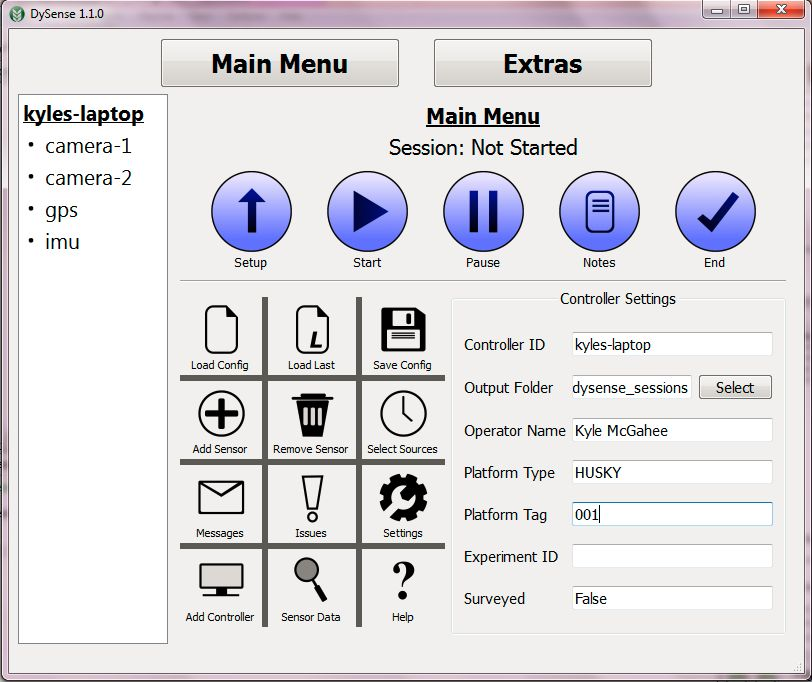
\includegraphics[height=4.5in]{figures/dysense2.png}
    \caption[Data collection program]{Screenshot of the data collection program.}
    \label{dysense_screenshot}
\end{figure}

DySense also uses GPS and IMU drivers to record the platform's position and orientation.  This knowledge of the platform state, as well as the camera offsets in the platform frame, allows the positions and orientations of each camera to be calculated at the same time as every image.    

\section{Additional Markers}
\label{system-markers}

In addition to the group QR codes there are two other types of markers used in the mapping process, row markers and plant markers.   

\subsection{Row Markers}

Row markers are placed at the beginning and end of each row. Similar to identifying plant groups, these markers are also implemented using QR codes.  These row codes store the row number and signify whether the code is the start ("St") or end ("En") of the row. As discussed in section \ref{section:plantid}, it is critical to know the planting direction of each row because that defines which plants are associated with each group QR code.

\begin{figure}[htb]
	\centering
    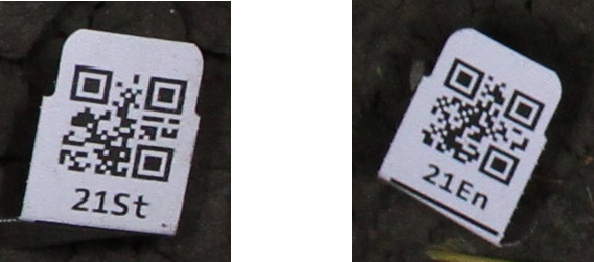
\includegraphics[height=2in]{figures/row_codes.png}
    \caption[Row QR codes]{QR codes marking the start and end of row 21.}
    \label{figure:row_codes}
\end{figure}

\subsection{Plant Markers}
\label{section:plant_markers}

The second type of marker is used to help distinguish regular plants from other plant debris that may be found in the field after tilling.  This marker is optional, but helps improve the robustness of locating plants.  Depending on the size and quality the field these markers can be used on every plant or, for example, every 4 plants. 

The marker used in this experiment is a blue dyed wooden stick approximately 5 inches in length, which is placed in the center of each plant. The color blue is selected because it provides the largest difference between other hues likely found in the field, such as yellow/green in plants and red in soil.  In addition to marking the plants, this stick also helps prevent the plants from flipping over when exiting the planter.

Another type of plant marker worth mentioning is a colored tag pierced through the top of an un-dyed wooden stick.  This type of marker can provide addition information for manual plant inspection and is much more saturated than the dyed sticks, making it easier to detect. 

\begin{figure}[htb]
	\centering
    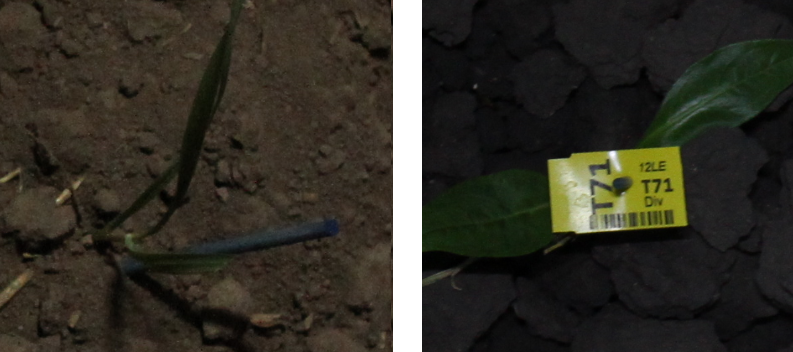
\includegraphics[height=2.5in]{figures/plant_markers.png}
    \caption[Plant markers]{Examples of blue stick (left) and colored tag (right)}
    \label{figure:plant_markers}
\end{figure}


\cleardoublepage

\chapter{Post-Processing Pipeline}
\label{chapter:pipeline}

After the images are collected they must be converted into a field map. This task is accomplished by a set of scripts that are run in a sequential, or pipeline, fashion, where the output of one script is used as the input to the next.  This chapter provides a general overview of the post-processing pipeline followed by a detailed explanation of each step.

\section{Pipeline Overview}
\label{processing-overview}

In this pipeline each script is referred to as a stage, where each stage accomplishes one specific task.  The main reason the post-processing is split into separate stages is several stages take a significant amount of time to run, so it's beneficial to not re-run the entire pipeline when changes are made to one stage.  The task that each stage accomplishes is:

\begin{description}
\item[Stage 0] Calculate the position and orientation of each image.
\item[Stage 1] Find and read \ac{qr} codes in all images.
\item[Stage 2] Determine the row structure of the field using the \ac{qr} codes.
\item[Stage 3] Detect leaves and plant markers in each image.
\item[Stage 4] Cluster plant parts from stage 3 into possible plants, and filter out unlikely plants.
\item[Stage 5] Assign individual numbers to plants and save the final field map to a file. 
\end{description}
 
The output of each intermediate stage consists of objects that directly relate to the field, for example \ac{qr} codes, plants, or rows.  These objects are serialized into a single output file which makes it trivial to pass these objects from one script to another. 

Every stage of the pipeline is written in the Python programming language, and all of the image-processing algorithms are performed using the Open Source Computer Vision library, also known as OpenCV.  The location of the post-processing code is listed in Appendix \ref{appendix:code_repositories}.

\section{Stage 0 - Calculating Camera State}
\label{processing-stage0}

The first step in the post-processing pipeline is to calculate the camera's position and orientation when each image was taken.  This is performed by the data collection program since it is a general process that's useful for many other types of sensors in addition to cameras.  However, after this calculation is done the format of the camera position is in latitude, longitude, altitude, and the format of the orientation is Euler angles.  Therefore, this initial stage must convert the camera position to the modified \ac{utm} coordinates discussed in Section~\ref{section:utm}, as well as calculate the homography matrix defined by equation \ref{equation:homography}.  

Even though the modified UTM coordinates use the ground reference for the z component, the height above the ellipsoid is also tracked for each image and item mapped in the field.  This information could be used to estimate relative differences in water content in different parts of the field due to changes in elevation. 

\section{Stage 1 - Extracting QR Codes}
\label{processing-stage1}

The initial goal after calculating the position and orientation of each image is to detect and read all \ac{qr} codes in the image set.  This process consists of four steps which are applied to every image.

\subsection{Converting Color-Spaces}

The first step is to convert the image from the default color-space, which is \ac{bgr}, to the \ac{hsv} color space.  As can be seen in Figure~\ref{figure:color_spaces}, this \ac{hsv} space is a cylindrical coordinate system which separates image intensity from color information.  This makes colors more robust to changes in lighting, and the angular hue component is better suited for describing how humans perceive the color spectrum.

\begin{figure}
	\centering
    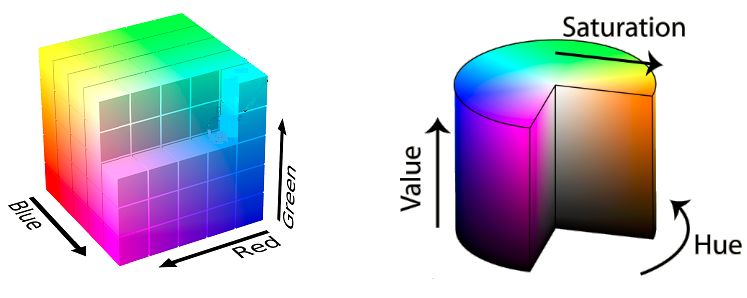
\includegraphics[width=5.5in]{figures/bgr_and_hsv.jpg}
    \caption[BGR and HSV color spaces]{Visualization of \ac{bgr} (left) and \ac{hsv} (right) color spaces. Images obtained under the Creative Commons License from the Wikimedia Commons.}
    \label{figure:color_spaces}
\end{figure} 

An important consideration is that most digital cameras perform a gamma-encoding when processing data from the imaging sensor.  This is a non-linear operation which maximizes the amount of intensity information that can be stored for each pixel, as it pertains to human perception.  However, human perception is not a valid concern in this post-processing application, and these non-linearities should be removed by properly decoding each color component.  This was not realized until after the research was completed, and thus it is not implemented in the pipeline.

\subsection{Thresholding}
\label{section:qr_thresholding}

The second step is to separate the white \ac{qr} codes from the rest of the image.  This is accomplished by applying a range threshold for each of the \ac{hsv} components.  This threshold will output a 1 (white pixel) if the all three components are in the specified range, otherwise it will output a 0 (black pixel).  In OpenCV hue is defined in the range of 0 to 179, and both saturation and value have a range of 0 to 255.  The range that was experimentally determined for separating \ac{qr} codes is shown in Table~\ref{table:qr_hsv_ranges}.

\begin{table}
    \begin{center}
    \caption[QR code detection values]{HSV range for detecting \ac{qr} codes.}
    \begin{tabular}[c]{|c|c|c|c|}
        \hline
        Component & Min Value & Max Value & Notes \\
        \hline
        Hue        & 0   & 179 & Include all hues      \\
        Saturation & 0   & 65  & Avoid saturated colors  \\
        Value      & 160 & 255 & Avoid dark colors       \\
        \hline
    \end{tabular}
    \label{table:qr_hsv_ranges}
   \end{center}
\end{table}

This threshold results in a binary image where pixels that are mostly white, such as \ac{qr} codes, are all white, and everything else is all black.  An example of a thresholded image can be seen in Figure~\ref{figure:code_extraction}.

\begin{figure}
	\centering
    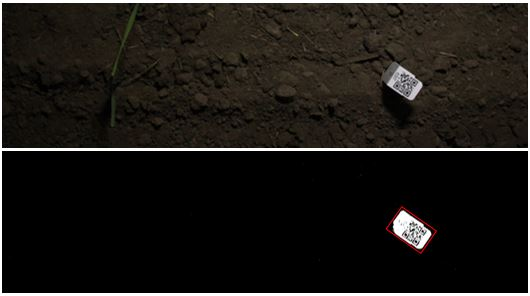
\includegraphics[width=5in]{figures/code_extraction_step1.jpg}
    \caption[Thresholded image]{Binary image resulting from the \ac{hsv} range filter.  The overlaid red rectangle shows the rotated bounding box associated with \ac{qr} code.}
    \label{figure:code_extraction}
\end{figure} 

\subsection{Filtering by Bounding Boxes}

The third step is finding the set of external contours, or outermost edges, of each object in the binary image.  Each set of contours is then assigned a minimum bounding box which is the smallest rotated rectangle that encompasses the entire object.  An example of a bounding box can be seen as a red rectangle in Figure~\ref{figure:code_extraction}.  These bounding boxes are filtered to remove ones that are either too small or too large to possibly be a \ac{qr} code.

\subsection{Reading QR Codes}
\label{section:reading_codes}

The final step is to use these bounding boxes to extract sections of the original image to run through the code reading program.  From the open-source programs that were evaluated, the ZBar program provided the best results.  However, the ZBar program requires a grayscale or binary image, and thus a threshold must be applied to the extracted color image. 

\begin{figure}
	\centering
    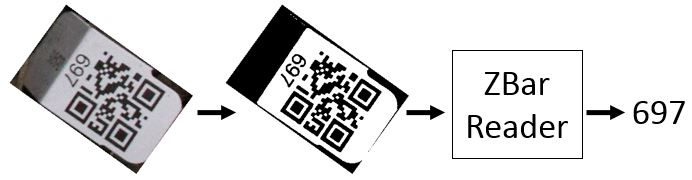
\includegraphics[width=6in]{figures/code_extraction_step2.jpg}
    \caption[Extracted code threshold]{Sequence of steps applied to objects that are potential \ac{qr} codes.  First a global or adaptive threshold is applied, and then the ZBar program returns the text stored in the code. In this case it would return 697.}
    \label{figure:code_extraction2}
\end{figure} 

The \ac{hsv} range threshold is effective for finding possible codes, but it does not do a good job maintaining the grid of white and black squares that make up the \ac{qr} code.  Instead, the \ac{bgr} image is converted to an intensity image, and if a simple global threshold does not result in a successful reading of the code then an adaptive threshold is tried instead.  This results in a readable code even if there is noticeable image glare as seen in Figure~\ref{figure:adaptive_threshold}. 

\begin{figure}
	\centering
    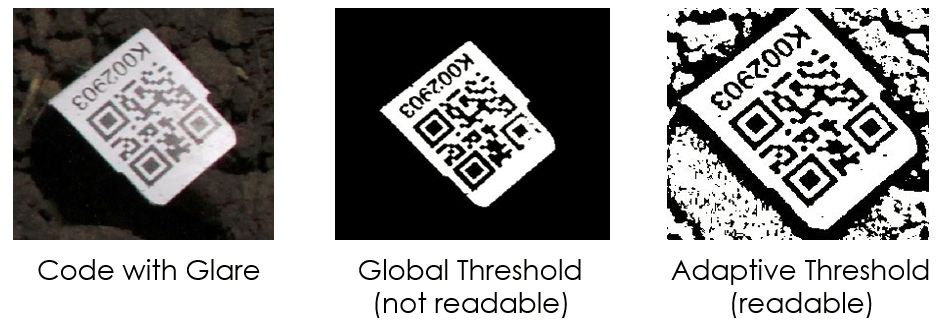
\includegraphics[width=5.5in]{figures/adaptive_threshold.jpg}
    \caption[Adaptive threshold]{Comparison showing how an adaptive, rather than a global, threshold can make a code readable by keeping the bottom right corner intact.}
    \label{figure:adaptive_threshold}
\end{figure} 

The data returned by the ZBar program is used to determine if the code corresponds to a plant group or to a row marker.  If no data, or bad data, is returned by the ZBar library then the extracted image is saved for the operator to review after the stage has completed.  This makes it much easier to find misread or damaged codes and to manually add them into the final results.  If the code is read successfully then its world coordinates are calculated and saved in a list of \ac{qr} codes.   If the same code is detected in multiple images then the world coordinates of each code reference are averaged to improve the mapping accuracy.

\section{Stage 2 - Creating Field Structure}
\label{processing-stage2}

The second stage of the pipeline involves assigning row numbers to each \ac{qr} code, and then creating plant groups that can span multiple rows.  As an optional input to this stage the user can specify a file containing any codes from the previous stage that were not automatically detected.  

\subsection{Assigning Codes to Rows}

This stage begins by pairing the row markers associated with the start and end of each row.  Since the locations of the marker codes are calculated from the images, the average row heading can be calculated.  This row heading is then used to transform the \ac{utm} coordinates into the field coordinate frame discussed in Section~\ref{section:field_coordinates}.

The next step is to assign each group \ac{qr} code to a specific row based on its field coordinates.  As some rows can span several hundred meters, it's not always possible to assign a code to the nearest row defined by a vector between the row start and end codes.  Instead a sweeping algorithm is used.   The idea is to sweep across the field, from left to right, and incrementally add \ac{qr} codes to each row as shown in Figure~\ref{figure:sweeping_algorithm}. Once a code is added to a row it splits that row into smaller segments.  A code is assigned to the row which has the closest segment based on the lateral distance to the code's field location. 

\begin{figure}
	\centering
    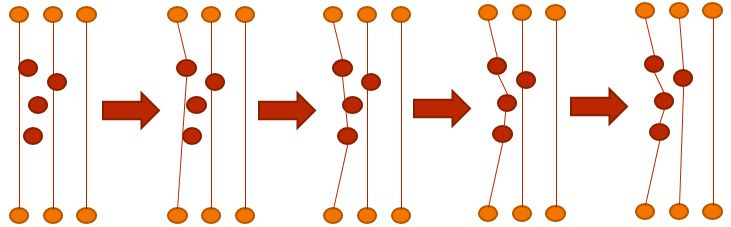
\includegraphics[width=6in]{figures/sweeping_algorithm.jpg}
    \caption[Sweeping projection algorithm]{Example of the sweeping projection algorithm. Row codes are shown in orange and four group codes in red.  At each step the left-most group code is assigned to the nearest segment, shown as a red line.  The result is three codes belong to the left row, and the fourth group code belongs to the middle row.}
    \label{figure:sweeping_algorithm}
\end{figure}

This algorithm can effectively account for small amounts of curvature in the rows, but it is not designed to work on rows that are not planted in nominally straight lines.

\subsection{Organizing Group Segments}

Once all group codes are assigned to a row, it's possible to tell which codes come before and after one another.  A group segment is defined by a beginning code and the next code that follows it in the direction of planting.  This group segment is where the plants for a given code are located.  It's possible, however, that when the transplanter reaches the end of a row that the current plant group isn't finished and continues into the next pass.  A pass refers to the transplanter driving once down the field, so a 2-row transplanter would have a pass containing 2 rows.  Therefore, the group segments at the end of corresponding rows are paired together into complete groups.  An example of this is shown in Figure~\ref{figure:group_segments}.

\begin{figure}
	\centering
    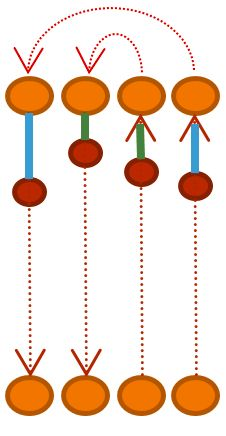
\includegraphics[height=2in]{figures/group_segments.jpg}
    \caption[Group segments]{Example of four rows planted two rows at a time.  The red dashed arrows show the direction of planting.  There are four group segments, two blue and two green.  The blue segments belong to the same plant group, and the green segments belong to a second plant group.}
    \label{figure:group_segments}
\end{figure}

\section{Stage 3 - Extracting Plant Parts}
\label{processing-stage3}

Similar to the process of extracting \ac{qr} codes, this stage converts each image to the \ac{hsv} color space, applies a range threshold, and filters the objects based on size.  Since this stage is looking for plant leaves rather than white \ac{qr} codes, it uses different ranges for the \ac{hsv} components.  These alternate ranges are defined in Table~\ref{table:plant_leaves_hsv_ranges}.

\begin{table}
    \begin{center}
    \caption[Plant leaf detection values]{\ac{hsv} range for detecting plant leaves.}
    \begin{tabular}[c]{|c|c|c|c|}
        \hline
        Component & Min Value & Max Value & Notes \\
        \hline
        Hue        & 35  & 90  & Include green hues        \\
        Saturation & 80  & 255 & Include saturated colors  \\
        Value      & 20  & 255 & Avoid very dark colors    \\
        \hline
    \end{tabular}
    \label{table:plant_leaves_hsv_ranges}
   \end{center}
\end{table}

In addition to plant leaves, this stage also searches for plant markers.  The values for the two types of markers discussed in Section~\ref{section:plant_markers} are shown in the tables \ref{table:stick_hsv_ranges} and \ref{table:tag_ranges}.  The minimum saturation and value for the tag markers can be set much higher than the wooden blue sticks which leads to more reliable detection.   

\begin{table}
    \begin{center}
    \caption[Blue stick detection values]{\ac{hsv} range for detecting blue stick markers.}
    \begin{tabular}[c]{|c|c|c|c|}
        \hline
        Component & Min Value & Max Value & Notes \\
        \hline
        Hue        & 90  & 130 & Include blue hues        \\
        Saturation & 31  & 255 & Include saturated colors  \\
        Value      & 16  & 255 & Avoid very dark colors    \\
        \hline
    \end{tabular}
    \label{table:stick_hsv_ranges}
   \end{center}
\end{table}

\begin{table}
    \begin{center}
    \caption[Yellow tags detection values]{\ac{hsv} range for detecting yellow tags.}
    \begin{tabular}[c]{|c|c|c|c|}
        \hline
        Component & Min Value & Max Value & Notes \\
        \hline
        Hue        & 15  & 45  & Include yellow hues       \\
        Saturation & 130 & 255 & Include saturated colors  \\
        Value      & 100 & 255 & Avoid dark colors         \\
        \hline
    \end{tabular}
    \label{table:tag_ranges}
   \end{center}
\end{table}

Similar to the \ac{qr} codes these values are set based on experimentation.   Unfortunately, good values for these thresholds are more likely to vary due to changes in external lighting or camera settings.  This is because they depend on finding specific colors, rather than white.  

\section{Stage 4 - Locating Plants}
\label{processing-stage4}

The most challenging aspect of the pipeline is reliably determining which plant parts found in the previous stage belong to the same plant, and which of those are actual plants that should be mapped.  Plant parts refers to both the leaves of the plant as well as any plant marker associated with the plant.  This is challenging because there is often unavoidable plant debris in the field that comes from the tilling right before planting. Plant markers, such as the blue sticks, help with this issue, but as discussed in Section~\ref{section:plant_localization} the blue sticks could not always be detected.  In addition, for large experiments it may not always be feasible to have individual markers for every plant.  

\subsection{Hierarchical Clustering}

The task of grouping plant parts into individual plants is done using a hierarchical clustering algorithm.  In this application a cluster is represented by the minimum bounding rectangle of one or more plant parts.  If two rectangles are clustered together the resulting cluster is represented by the smallest bounding rectangle that fits both the original rectangles.  For simplicity the merged rectangle is a regular, non-rotated bounding rectangle. 

This algorithm combines the nearest two clusters into a single cluster and keeps repeating this process until an end condition is met.  The distance between two clusters is defined to be the smallest distance between any of the 4 rectangle corners.  The end conditions are either (1) there is nothing left to cluster, or (2) the closest cluster is too far apart to be merged based on a user defined threshold.  In addition, there is a maximum size limit on the clusters which is set to be the maximum expected plant size in the field.  Finally, any tiny, unclustered plant parts are removed from the list of possible plants. 

\begin{figure}
	\centering
    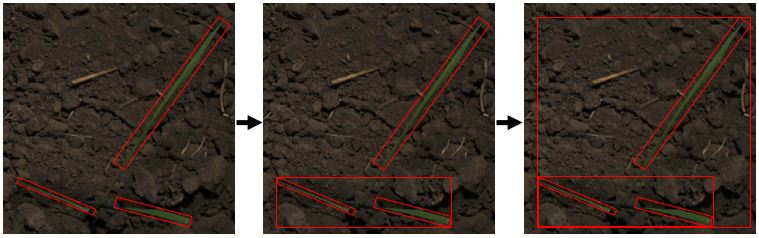
\includegraphics[width=5in]{figures/clustering.jpg}
    \caption[Hierarchical clustering]{Example of hierarchical clustering. At each step the closest bounding boxes are merged together until there is one containing the entire plant.}
    \label{figure:clustering}
\end{figure}

\subsection{Recursive Segment Splitting}

After the clustering is completed for an entire plant segment, the list of possible plants is passed to a recursive splitting algorithm to filter out the real plants.  This algorithm leverages information about the expected locations of plants as well as takes into account the plant markers found in stage 3.  The splitting algorithm consists of the following steps for each segment:

\begin{description}
\item[Step 1] For each possible plant, calculate the lateral and projection distance to the segment.  
\item[Step 2] Remove any plants that do not fall within the segment based on the projection distance.
\item[Step 3] Find the most likely plant based on various characteristics.  This is described in more detail below.  If there are no possible plants then create one in the next expected location based off the nominal transplanter spacing.  
\item[Step 4] Repeat the previous step, but starting at the end of the segment and find the next most likely plant by working backwards.
\item[Step 5] Split the original segment into smaller segments using the most likely plants as new endpoints.  If the new segments are too short to contain plants then the algorithm is finished.  Otherwise, recursively go back to step 1 for each of the new segments.
\end{description}

The idea behind working from the both directions at the same time is the start and end \ac{qr} codes are known locations in the field, and thus plants near them can be more reliably detected.  In order to determine the most likely plant in step 3, each possible plant is assigned a penalty value.  This value is calculated using

\begin{center}
Penalty = ($s_L$L + $s_P$P + $s_C$C) / ($s_B$B)
\end{center}
where the variables are described below.

\begin{description}
\item[Lateral Error (L)] How far off the plant is from the expected line segment.
\item[Projection Error (P)] How far away the plant's projection onto the segment is from where the closest expected plant would be.
\item[Closeness (C)] How far away the plant is from the start/end of the segment, with the idea that the lateral and projection errors become less reliable the farther away the plant is from a known item's location.
\item[Plant-Part Boost (B)] Based on what types of plant parts are found in the plant cluster.
\item[Scales ($s_L,s_P,s_C,s_B)$] Relative weightings to change importance of each penalty.
\end{description}

The individual penalty components are calculated with the piece-wise linear functions displayed in Figure~\ref{figure:piecewise_penalties}.  The plant-part boost (B) is calculated as a product of additional scales for each plant part type.  If a certain type of plant, for example a blue stick, is missing from a possible plant, then its scale is set to 1 so that it has no effect.  

\begin{figure}
	\centering
    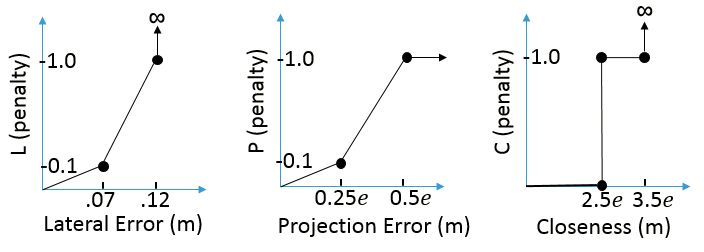
\includegraphics[width=5.5in]{figures/piece_wise.jpg}
    \caption[Penalty functions]{Piece-wise penalty functions. "$e$" represents the expected spacing between successive plants.}
    \label{figure:piecewise_penalties}
\end{figure}

The lateral and closeness penalties are defined as infinity if the input exceeds a certain threshold.  If this occurs then the overall penalty will also be set to infinity, and that plant will be removed from the list of possible plants.  If this results in no plants to select from then a plant will be created and placed in the expected location.  These are referred to as "Created Plants", and may occur due to a plant being dead, buried, or skipped during planting.  

A simple example of the algorithm is shown in Figure~\ref{figure:recursive_algorithm}.  In the first image there is one segment between the two \ac{qr} codes.  The second image shows the result of the splitting algorithm running on segment labeled \#1. It selects one plant based on the bottom code and one based on the top code.  Segment \#2 is determined to be too short to contain more plants, however the algorithm is recursively run again on segments \#3 and \#4.  This results in the third image, which now contains five segments.  One plant had to be created because the other two possible plants on segment \#3 had too much lateral error to be considered.   

\begin{figure}
	\centering
    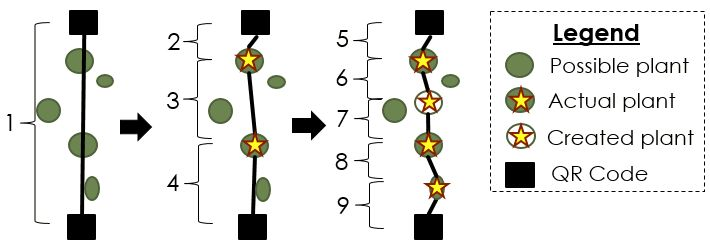
\includegraphics[width=5in]{figures/recursive_algorithm2.jpg}
    \caption[Recursive splitting algorithm]{Example of the recursive splitting algorithm finding most likely plants within a group segment.}
    \label{figure:recursive_algorithm}
\end{figure}

Similar to the sweeping projection algorithm used to assign row numbers, this algorithm can effectively account for slight curves within a group segment since plants are incrementally determined starting at the end points. 

\section{Stage 5 - Saving Field Map}
\label{processing-stage5}

The final stage in the pipeline is generating a field map file.  This stage begins by assigning every plant in the field a unique number so it can be easily referenced in a database.  This numbering begins with plant \#1 at the start of the first row and then follows a serpentine pattern which can be seen in Figure~\ref{figure:serpentine}. This numbering system is chosen because it represents how a person is likely to inspect plants when walking through the field.  

One complication that is addressed in this final stage is that there may be a relative shift between the coordinates calculated by the mapping platform and the desired coordinates.  This is due to the fact that \ac{rtk} systems are only accurate relative to the base station.  If the location of the base station isn't accurately surveyed then the field map will contain an offset in the both the northing and easting directions. 

In order to account for this offset, a file can be provided as input to the stage that contains the coordinates of surveyed \ac{qr} codes relative to the desired reference station.  The average offset between these surveyed codes and the mapped codes is computed and every item in the map is translated by this amount. After this correction is complete all the codes and plants are written to a \ac{csv} file.  This is a common type of file and can be used with many types of programs, or it can be easily imported into a database.

\begin{figure}
	\centering
    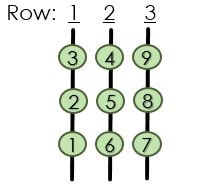
\includegraphics[height=1.7in]{figures/sepentine.jpg}
    \caption[Serpentine numbering]{Example of serpentine numbering for nine plants.}
    \label{figure:serpentine}
\end{figure}


\cleardoublepage

\chapter{Experimental Setup}
\label{experiment}

The mapping process was evaluated at the Land Institute on a type of intermediate wheat grass (IWG), commonly referred to as Kernza.  The Land Insttitute is one of the worlds leading researchers in perinial agriculture focusing on <>. This experiment involved

%5.1.1.	Crop type, time of year, location, researcher, etc 

\section{Field Setup}
\label{experiment-field}

A transplanter, shown in figure TODO, was used to plant two rows a time.  The transplanter works by a series of six deposit cylinders rotating at a constant rate.  When <> hits a plant is ejected, a small amount of water is applied to the plant and the rolling wheels help press the soil down around the plant.  

The six deposit cylinders rotate so that each cylinder is spaced 12 inches apart.  Plants are placed in every other cylinder which results in 24 inches between successive plants.  The QR codes indicating the start of a new group are placed in the empty cylinders between two plants, which means the use of QR codes does not increase the overall size of the field. 
 
The spacing between each row on the transplanter was 36 inches. 

The field consisted of approximately 25,000 plants split into 97 individual rows.  After the field was planted the QR code marking the start and end of each row were manually placed.

%5.1.4.	Figure of transplanter.  

\section{Mapping Window}

An important decision is whether to map during the day or at night.  The biggest challenge of mapping during the day is the ability to provide consistent lighting.  Changes in scene lighting, for example between clouds and direct sun, can affect the color of plants and blue sticks and potentially cause under or over-exposure of QR codes.  Daytime lighting can be made more consistent by using a shade cover over the field of view of the images.  However this depends on the sun being high enough in the sky for the shading to work, which limits the total amount of time images can be collected each day.  

The shade size can always be increased or placed at an angle to account for the sun angle, however this increases cost, design complexity and makes the platform more susceptible to wind gusts.  

This limited time window 





% Importance of mapping before it rains.
%5.2.3.	Mapping at nighttime vs. daytime.   Importance of shade.

% Not enough high-sun lighting during day to use umbrellas.
% Need to map before it rains.  
% Easier to have free time at night.

% Include equation for shade. 
% Include figure for shade.  

\section{Camera Setup}

An important step in ensuring the mapping process is robust is choosing the correct camera options. 

''' delete ? '''
 Some of these options will vary in how they're determined between day and night-time mapping, because at night the available light is much more restricted.  Since night-time 
''''

The first option selected is the shooting mode, as that defines what settings are available to change.  The preferred shooting mode is Manual since that will allow the exposure time, aperture and sensitivity to be set to constant values.  Under controlled lighting conditions this will keep a consistent scene luminance and prevent any additional latency due to the camera calculating these settings before exposing a new image.

The maximum exposure time is determined based on the speed of the robot and maximum allowed translation in the QR codes.  If the exposure time is set too high the black and white squares making up the QR codes will start to blend together and the code will be unreadable.  

<TODO> put in equation 

The aperture is set to a large diameter to maximize the amount of luminance since the exposure time is relatively short for the amount of light available.  However when the lens is fully open, an f-stop of f/2.8, the depth of field is noticeable reduced and it becomes more difficult to keep the QR codes in focus as the camera slightly varies in height as it moves through the field.  Therefore an f-stop of f/4 was chosen which provides a good trade-off between depth of field and luminance.  Also compared to f/2.8, an aperture of f/4 will have less noticeable lens effects such as distortion and vignetting which will result in higher quality images.  

The light sensitivity of the sensor, commonly specified as an International Standards Organization (ISO) rating, is set last by inspecting the image in the field to achieve a desirable scene luminance.  Using the two LED bars per camera required an ISO of 1000.  If the ISO is set too high then sensor noise becomes significant which decreases the robustness of the mapping.  If too high of an ISO is required, then the aperture can be made larger or by adding more external light sources.  

The white-balance is set to a fixed setting chosen to match the same color of light as the LED bars, which is listed as 6000 Kelvins.  Many cameras offer both a Flash and Cloudy white balance which are both centered around 6000K.   Preliminary field tests indicate both options produce very similar results, so the Flash setting was used.   

Auto-white balance mode should not be used as most images will not contain a QR code for reference and as a result many images of plants will vary in chromacity. 

Finally the image format is selected between raw and the Joint Photographic Experts Group (JPEG) format.  Raw images store the pixel readings directly from the sensor, thus no information from the exposed image is lost.  The JPEG format on the other hand typically merges adjacent pixels from the Bayer filter and applies a compression algorithm to reduce the file size.  Even though the compression algorithm produces image artifacts and reduces the quality of the QR codes, this does not reduce the effectiveness of the post-process pipeline. For the Canon 7D camera, raw image are around 15 megabytes (MB) larger and require a conversion to a bitmap format before being useful for post-processing.  This format conversion requires approximately 5 to 10 seconds per image and adds a significant amount of time to the post-processing pipeline.  For these reason the JPEG format is used for mapping.

\section{Robot Operation}

In section <TODO> it was discussed that the robot can operate in either cruise control mode or a fully autonomous mode.  In this experiment the robot was used in cruise control mode, mainly because at the time there were not any tools available to view and edit the waypoints used by the robot.  When generating a set of waypoints from the transplanter path, the waypoints at the row ends need to be edited to prevent the robot from driving in too rough of field conditions, and also to prevent from turning before the end of the row and running over plants. 

Even though the robot was operating in cruise control mode, the path of the robot was recorded and it's possible to have the robot retrace this path in autonomous mode.  This is useful for autonomously collecting plant data which is used for monitoring plant traits such as height or greenness.


\cleardoublepage

\chapter{Results and Analysis}
\label{processing}

\section{Code Detection}

From the 4581 codes in the field, all but 2 were automatically detected by the first stage of the post-processing pipeline.  However 43 codes were not able to be read by the ZBar program.  It is unknown why the 2 undetected codes were not detected, but the most likely reasons are they were accidentally buried or they did not appear in any images.  

Since each of the unreadable codes were placed in a special review directory as described in section <TODO> it was straightforward to determine the reason each code couldn't be read.  The most likely cause was a printer error which caused a small section of the code to not be printed.  This printer error affected 25 of the 43 unreadable codes.  9 codes were partially blocked by field debris or insects sitting on the code.  7 had dirt on the code, which most likely splashed up during transplanting. And finally 2 codes were too blurry too be read successfully.  Examples of each of these issues can be seen in figure TODO. 

The codes affected by printer error could be reduced by better inspecting the codes before planting or by using a different type of printer.

%6.2.	 figures of each unreadable codes

\section{Plant Localization}

Before planting the number of plants in each group were manually counted. However, it is unknown exactly how many plants ended up in the field because some plants were discarded during the transplanting process.  So the sum of the pre-counted plants, 25560, is the maximum number of plants that could be found in the field.  

The plant localization algorithm detected 24269 plants in the images and created 335 plants where no plant was detected, but where one should have been.  This resulted in a total of 24604 plants in the final map indicating 956, or roughly 1 out of every 25, plants were discarded during transplanting.  For this experiment these results were considered reasonable. 

Blue sticks were only found in 23\% of the plants that were detected in the images, however all plants should have had a blue stick marker.  The reason for this poor result was due to the lack of saturation in the blue sticks which made it difficult to find a threshold that didn't also detect the blue hues in the soil.  

% TODO how to find blue stick problem. 

The assigned coordinates of the creates plants were projected back onto images that contained those world coordinates, and an arbitrary 10 centimeter box was drawn on the image to indicate where the plant should have been.  Fifty of these debug images were manually analyzed and 47 of them closely matched an actual plant in the image that was either dead or partially buried under soil.  The remaining 3 plants were either completely buried or more likely a gap occurred in the field where no plant exists.  

\section{Mapping Accuracy}

As discussed in section <TODO>, the coordinates of all the plants and QR codes had to be offset into the coordinate frame used by the Land Institute.  This was accomplished by manually surveying 10 codes using the Land Institute receiver and base-station and then calculating the northing and easting offsets that would make the average error zero.  

After this offset is applied, the error of the 10 surveyed codes was calculated and can be seen in figure <TODO>.  The line of best fit runs through the origin and shows that the average error is indeed zero.    

% TODO figure of errors showing each code as point on easting/northing error plot.

The reason that codes were used to calculate the offset, rather than plants, is it's much easier for the post-processing to consistently identify the center of the code. 

An additional 20 plants were surveyed to verify that their mapped positions were accurate enough to distinguish them from their neighboring plants.  All surveyed codes and plants were chosen randomly and evenly distributed throughout the field which indicates these errors are representative of all plants.   A similar plot showing the errors for each surveyed plant can be seen in figure <>.  The average error was <> which indicates the offsets calculated using the codes weren't biased.  The maximum errors in the easting and northing directions are <> and <>, respectively.  

TODO are these errors small enough?



The biggest source of errors from these measurement are errors in assigning an accurate time-stamp to each image.  These timing errors are primarily caused by camera latency and latency in the GNSS receiver.  Camera latency is the amount of time between when the data collection program commands the camera to take an image, and when the image is actually exposed.  GNSS latency is the amount of time between when an a position is calculated by the receiver, and when it is received by the data collection program.  

TODO show that these errors are same order of magnitude.

The forward motion of the robot was primarily in the northing direction which explains why these errors are around twice as large as the easting direction.  

The additional errors in the surveyed plants compared to the codes is likely due to a larger discrepancy between what the post-processing pipeline detects as the center of a plant and what the human measures as the center of the plant. 

TODO talk about GPS accuracy?

\section{Plant Spacing}

An additional check to verify the results is that the plant spacing should be consistent with the output rate of the transplanter.  The histogram below shows the distribution of plant spacing for all the plants.  As expected the most common plant spacing is around 24 inches, however the variances in plant spacing highlights the importance of mapping individual plants, rather than assuming even spacing.

TODO insert histogram.

\section{Time Analysis}

An important consideration to the success of the mapping process is much time it takes to collect and analyze all of the images. For this experiment the robot speed and camera triggering rate were set as described in section <TODO>.  This resulted in a total driving time of approximately 10 hours spread over 4 different nights.  Each night required 30 minutes for setup and another 30 for tear-down, which resulted in a total of 4 additional hours.  

During the 10 hours of driving, the robot collected <> images.  The timing analysis for the post-processing are presented in table <TODO>. These results were bench-marked on a Lenovo S431 ultra-book running a dual core i7-3687 CPU at 2.6 gigahertz (GHz) with 8 gigabytes (GB) of random access memory (RAM).  

TODO insert table of stage timing.

One thing to note is it's straightforward to run the first stage in parallel for each night images were collected, since these are independent sessions.

TODO compare to manual survey


\cleardoublepage

\chapter{Conclusion}
\label{conclusion}

The results of this research show that the image-based mapping process is a viable option for locating and identifying individual plants.  For the experiment discussed in this paper, it is estimated that the image-based mapping allowed the field to be mapped four times faster <TODO> than traditional manual surveying, and with less tedious work.  The average error of 6 centimeters <TODO verify> is comparable to manual surveying errors, and the worse case error of 12 centimeters <TODO verify> is well within the maximum error allowed to differentiate adjacent plants.  The group identification method successfully located all but 2 QR codes, which is a success rate of 99.96\%.  While the mapping process was successful, other important conclusions regarding the platform, plant markers, cameras and system-complexities can be drawn from the research and are discussed below.

The image-based mapping is independent of the base platform is used, and the robot used in this experiment could easily be switched out for a simpler platform such as a manual push-cart.  A robot was used in this experiment based on the potential to automate the image collection step.  However, this research indicated two benefits of having a human present in the field during the image collection.  First is to detect if a camera stops taking pictures due to some error, and second is the ability to fix QR codes that are partially buried and covered by field debris.  The first issue could be mitigated by providing automatic feedback between the robot, user and data collection program and the second could be solved by walking through the field and fixing these codes before the robot drives itself through the field.  Both of these steps would be required for robust automated image collection.       

The least successful aspect of the experiment was the use of dyed blue sticks acting as plant-markers.  As discussed in section <TODO> these wooden sticks suffered from inconsistent <TODO> and didn't reflect enough light to appear saturated in the images.  An alternative option is to use colored, plastic square markers that are pierced through un-dyed wooden sticks.  To avoid large amounts of plastics being distributed in the field these markers would not need to be on every plant, but rather every 4 or 5 plants.  If there is very little field debris or weeds then these plant markers may not be necessary at all. 

The limiting factor on how quickly images could be collected was the maximum trigger rate of the Canon 7D cameras.  Additionally these cameras had an indeterminate latency that led to positional errors and suffered from occasional crashes with both the camera hardware and the software used to interact with the camera.  A potentially better option would be to use a camera originally designed to transfer images over the Universal Serial Bus (USB) and equipped with a high-resolution lens.  These cameras typically have much higher capture rates and were intended to be used for scientific or robotic applications, unlike the Canon's which were primarily intended for photographers. 

Perhaps the biggest conclusion drawn from the research is the importance of managing complexity in an application that is primarily intended to be used by researchers.  Using images adds complexity in the fact that camera settings have to be setup carefully, and the thresholds in the post-processing have to be chosen to work with both the chromacity and lumination of the images.  These thresholds can vary over multiple experiments due to slight changes in environmental lighting and it's difficult to find a set of values that work well for all scenarios.     

TODO mention trigger mapping with barcode scanner?

Regardless of what type of equipment is selected to collect images, this paper presents important first steps in creating a robust mapping process that will allow researchers to increase the size of their experiments. This will allow more variety in plant populations and an increase in the number of field repetitions among certain plant groups which will lead to better selection and faster refinement of.  


% +--------------------------------------------------------------------+
% | References
% +--------------------------------------------------------------------+

% +--------------------------------------------------------------------+
% | Included for Gather Purpose only.  Do NOT uncomment the next line.
%input "references.bib"
% | In order for the WinEDT editor to index references correctly, it
% | has to know where the "references.bib" file resides.  This
% | command will be ignored completely by LaTeX
% |
% | WinEDT can read file path names with either "\" or "/". LaTeX,
% | however,doesn't like "\", so it's easier to store a path name
% | using forward slashes "/".
% +--------------------------------------------------------------------+

\cleardoublepage
\phantomsection

% +--------------------------------------------------------------------+
% | This template uses the BibTeX program to format references.  The
% | lines below create a separate Bibliography section and add
% | an entry for "Bibliography" to the Table of Contents.  The actual
% | data for your references (author, title, journal, date, etc.) are
% | entered in the references.bib file.  See "Citations and Bibliography"
% | for details on to creating citations and formatting references.
% +--------------------------------------------------------------------+

\addcontentsline{toc}{chapter}{Bibliography}
\bibdata{references}
\bibliography{references}

% +--------------------------------------------------------------------+
% | The following commands add the appendices  To add or delete
% | appendices, add or remove the line
% |
% |     \input{appendixX.tex}
% |
% | where "X" is the letter designation of the appendix (A, B, C,
% | etc.) You should have one \input{appendixX.tex} line and a
% | corresponding file appendixX.tex for each appendix.
% |
% |If you do not have any appendices, comment out or delete the three
% |lines below.
% +--------------------------------------------------------------------+

\appendix
% +--------------------------------------------------------------------+
% | Appendix A Page (Optional)                                         
% +--------------------------------------------------------------------+

\cleardoublepage

\chapter{Title for This Appendix}

\label{Appendix:Key1}

Enter the content for Appendix A in the appendixA.tex file.  If you
do not have an Appendix A, see comments in the etdrtemplate.tex file
for instructions on how to remove this page.

% +--------------------------------------------------------------------+
% | Appendix B Page (Optional)                                         
% +--------------------------------------------------------------------+

\cleardoublepage

\chapter{Code Repositories}
\label{appendix:code_repositories}

\noindent \large Post-Processing Pipeline 

\noindent \url{https://github.com/Phenomics-KSU/HTMI}

\vspace{5mm}

\noindent \large Data Collection Program (DySense)

\noindent \url{https://github.com/DySense/DySense}

\vspace{5mm}

\noindent \large Extended Robot Functionality in ROS 

\noindent \url{https://github.com/Phenomics-KSU/htp_auto}

\vspace{5mm}

\noindent \large Trimble GPS Driver in ROS (htp\_auto branch)

\noindent \url{https://github.com/Phenomics-KSU/nmea_navsat_driver}



\end{document}

% +--------------------------------------------------------------------+
% | Template Revisions
% |
% | 9/14/06: Removed typos
% | 3/29/13: Removed hypernat package
% | 4/5/13: Changed to plain bib style
% | 5/17/13: added /cleardoublepage and /phantomsection to
% |          /bibliography to correct TOC page problem
% | 5/17/13: Fixed TOC problem with Dedication, Preface, etc.
% | 12/16/15: Added tocloft package to produce leader dots for all
% |           entries in the table of contents.
% |           Added geometry package to specify 1 inch margins.
% |           Removed unnecessary color specifications.
% |           Changed to \citep for citations.
% | 2/9/2016: Replaced \bibpunct with \setcitestyle.
% |           Changed to unsrtnat style
% |           Added natbib.pdf and Citations and Bibliography.pdf files
% |
% +--------------------------------------------------------------------+
